


  %\system, illustrated in Figure \ref{fig:system}, is a processor architecture which aims at providing secure code execution by means of \puf-based authentication of cache lines. The central idea behind \system~is a \puf-Tag (\ptag) Memory, which runs in parallel with the system main memory (Figure \ref{fig:system}). Each entry in the \ptag~Memory stores an authentication code of a cache line generated by a \puf-based device located on-chip.
  
%   \begin{figure*}[!ht]
% 	\centering
% 	\includegraphics[scale=0.35]{cshia}
% %	\vspace*{-12pt} 
% 	\caption{A system overview of the \system~system.}
% %	\vspace*{-9pt} 
% 	\label{fig:system}
% \end{figure*}

  %\new{In comparison to traditional architectures, \system~includes two main modifications: The \textit{Secure Engine} (\tagsystem), which includes the \textit{PTAG Generator} (\ptaggen, Figure \ref{fig:ptaggen}); and the \textit{Security-Cache} (\seccache) that controls bus traffic between the processor and the \textit{Memory Controller} (\mctrl). Other two new architectural components are also required to complete the \system~design, the \textit{\ptag~Memory} and the \textit{PTAG Bus}. In a few words, when the processor requires\slash{}sends data\slash{}instructions to the \mctrl, the \seccache~sends the related cache line to the \tagsystem~for computing\slash{}validating its \ptag. Notice from Figure \ref{fig:system} that the \ptag~bus runs in parallel to the system buses, and thus no program can directly read the \ptag~Memory, since neither the processor nor the \mctrl~are aware about the \seccache.}


  % \subsection{\ptaggen~Operation}
  % \label{subsec:ptaggenOpr}

  % \new{The \tagsystem~controls the \ptaggen~based on the information delivered by the \seccache. This information is generated from bus transactions (Memory READ, Memory WRITE and I\slash{}O) between the processor and the memory controller, and which the \seccache~controls. Next, each \ptaggen~action is explained in regard to bus transactions.}
  
  %     \begin{figure*}[!ht]
	 %  \centering
	 %  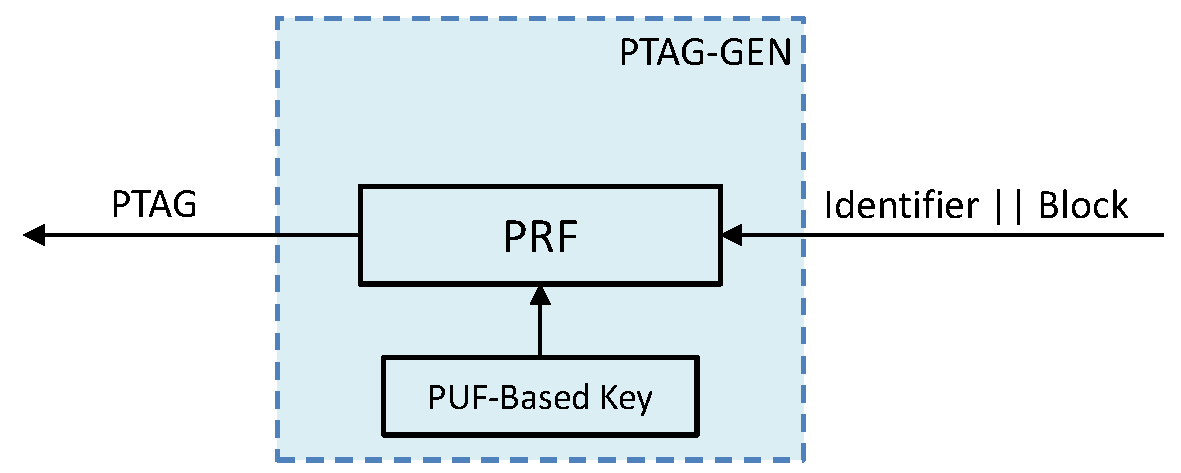
\includegraphics[scale=0.4]{ptaggen}
	 %  \caption{The \ptaggen~during \ptag~Generation (write) and \ptag~Verification (read) operations.}
  % %	\vspace*{-9pt} 
	 %  \label{fig:ptaggen}
  % \end{figure*}
  

	 %  \subsubsection{\ptag~Generation (memory write)}
	 %  \label{subsubsec:ptag-generation}
  % \new{During a write operation, the \seccache~passes data\slash{}instruction cache lines to the \tagsystem~and the \ptaggen~computes \ptags~and stores it into the \ptag~Memory. A \textit{Pseudorandom Function} (\prf) \cite{Goldreich2004} module is used to generate the \ptag~and takes as input the concatenation ($||$) of the cache line bits and the base address of the cache line provided by the core (see Figure \ref{fig:ptaggen}). In order to ensure uniqueness, the \prf~is configured using a \textit{unique-per-device key}. This key is produced by the intrinsic hardware features of a~\puf. Such authentication tag is specific to the core running that specific cache line, as ~\puf~outputs are dependent on the statistical variations of the manufacturing process, and are unique to each processor~\cite{Katzenbeisser2012}. Hence identical cache lines running on different processors will produce different \ptag~values for the same inputs. Notice that only code in the cache, for which integrity has been ensured, will be able to write to memory.}
  


	 %  \subsubsection{\ptag~Verification (memory read)}
	 %  \label{subsubsec:ptag-verification}
  % \new{During a read operation, the \seccache~passes data\slash{}instruction cache lines to the \tagsystem~and the \ptaggen~computes \ptags~for verification. As shown in Figure~\ref{fig:ptaggen}, during a read operation the cache line base address produced by the core is appended to the cache line contents read from memory and the result is fed to the \prf~module. The \ptag~produced this way is compared to the PTAG read from memory for equality. If the previously stored \ptag~and the recently computed value do not match, a \textit{Non-Maskable Interrupt} (NMI) is generated to the core (called \ptagnmi), as code\slash{}data integrity may have been violated. As shown in Figure \ref{fig:system}, in order to hide \puf~latency, the data\slash{}instruction is sent to the respective cache (I\$ or D\$) at the same time that \ptag-GEN computes the \ptag~for that cache line and compares it to its \ptag~previously stored into the \ptag~Memory.}

	 %  \subsubsection{Handling I\slash{}O}
	 %  \label{subsubsec:io}
  % In modern computer systems, I\slash{}O operations store data directly into specific memory regions through DMA mechanism. Thus, it is not possible to trust such memory regions and \system~does not ensure their integrity and authenticity. Software should first perform authentication of I\slash{}O data in a higher abstraction layer and then copy it to secure areas where the \system~can ensure integrity and authenticity.


%\mario{never start a chapter with a figure, Add an introduction about what is going to be explained in  this chapter }





\section{Overview}
\label{sec:overviewarch}

\mario {cite Caio thesis, make clear each contribution}
\cshia~was originally proposed in \cite{Hoffman2015} as an architecture for \iot. However, we believe that \cshia~fits in a broader class of embedded system applications that can benefit from its nice security features. Many embedded system applications do not need secrecy\slash{}confidentiality, but strongly require code and data authenticity and integrity. 
%\augusto{This is a detailed version with Caio  contribution   in a higher level, this work is about just authenticity so it would be better to  get the version to TECS and  talk about the  improvements made by caio and cite his thesis, i just dont know in which part }
\begin{figure}[!ht]
    \centering
%     \includegraphics[scale=0.45]{cshia}
    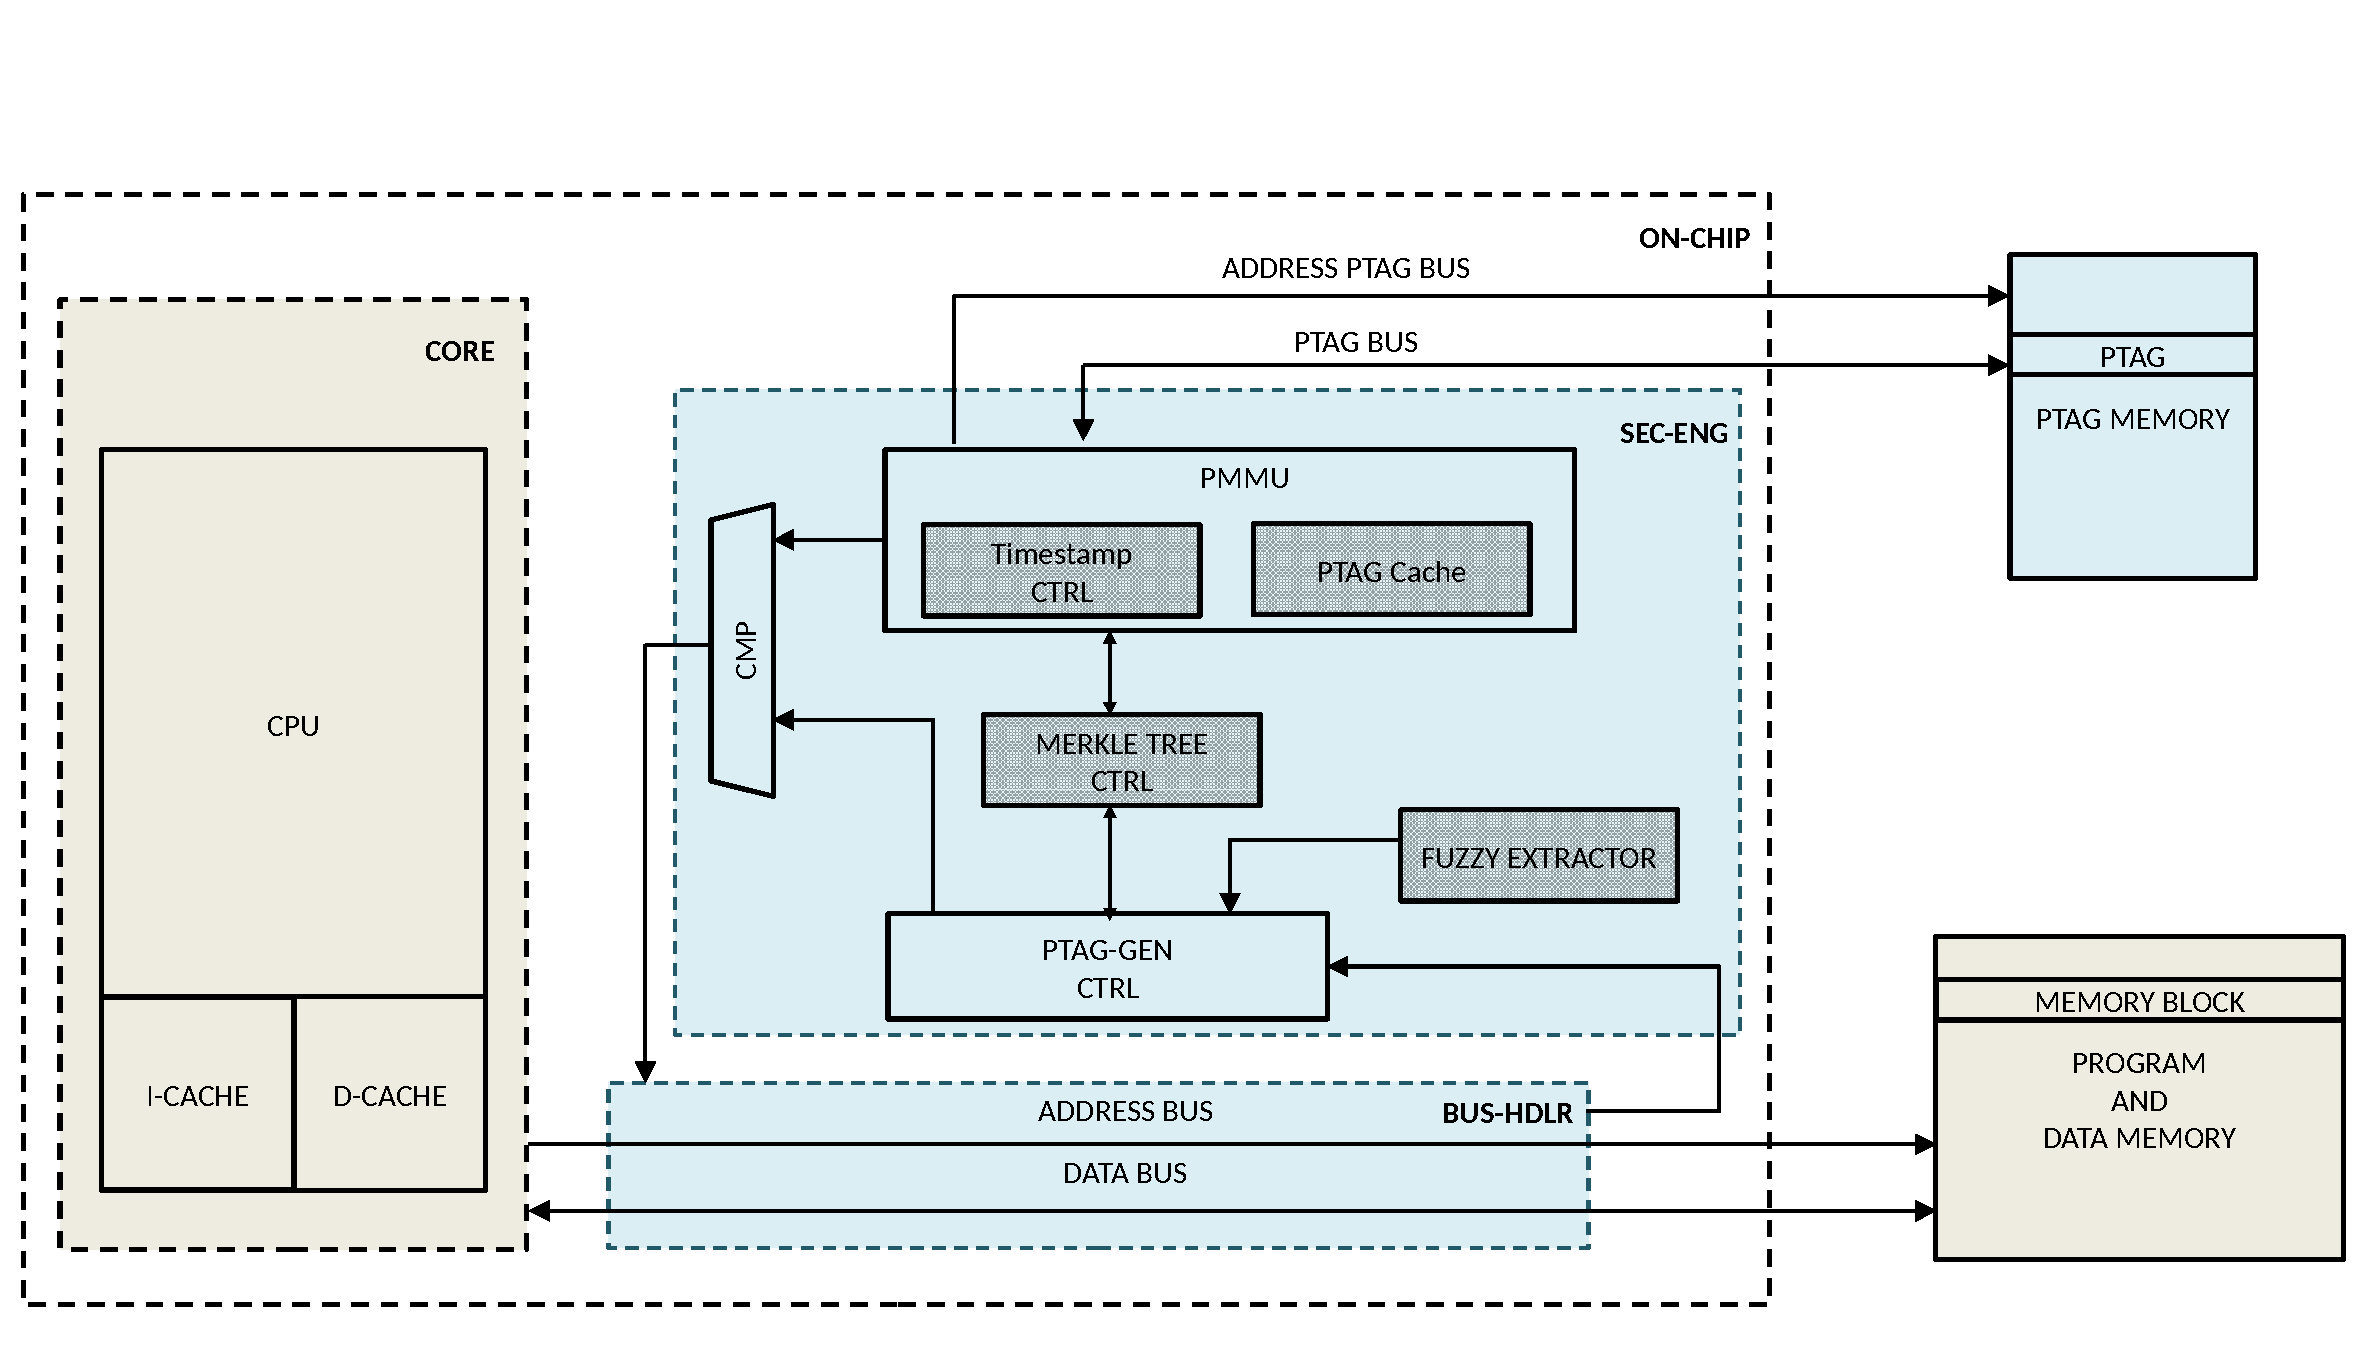
\includegraphics[width=\textwidth]{figures/pdf/CSHIA_detailed_caio_expansion.pdf}
    \caption{The \cshia~architecture.}
%    \vspace*{-9pt} 
    \label{fig:cshia}
\end{figure}
%\begin{figure*}[!ht]
%    \centering
%     \includegraphics[scale=0.45]{cshia}
%    \includegraphics[width=\textwidth]{figures/pdf/cshia.pdf}
%    \caption{The \cshia~architecture.}
%    \vspace*{-9pt} 
%    \label{fig:cshia}
%\end{figure*}
Using the original work with some architectural elements modified to provide stronger security features, the first LEON3 \fpga~ based implementation of \cshia was realized. This section focus on presenting the \cshia~implementation components and how they work to provide authenticity and integrity. Figure \ref{fig:cshia} illustrates the basic components required for \cshia~ to work: 
\begin{itemize}
    \item One core that in this implementation is a LEON3 processor;
    \item The \cshia~ components:
    \begin{itemize}
        \item \ptag~ Memory Management Unit (\pmmu)
        \item Bus Handler (\handler)
        \item Security Engine (\seceng) 
    \end{itemize}
    \item One external memory that contains instructions and data;
    \item One interconnection bus using \amba.
\end{itemize} 


\section{\amba}
\label{sec:amba2}
\begin{figure}[!ht]
    \centering
    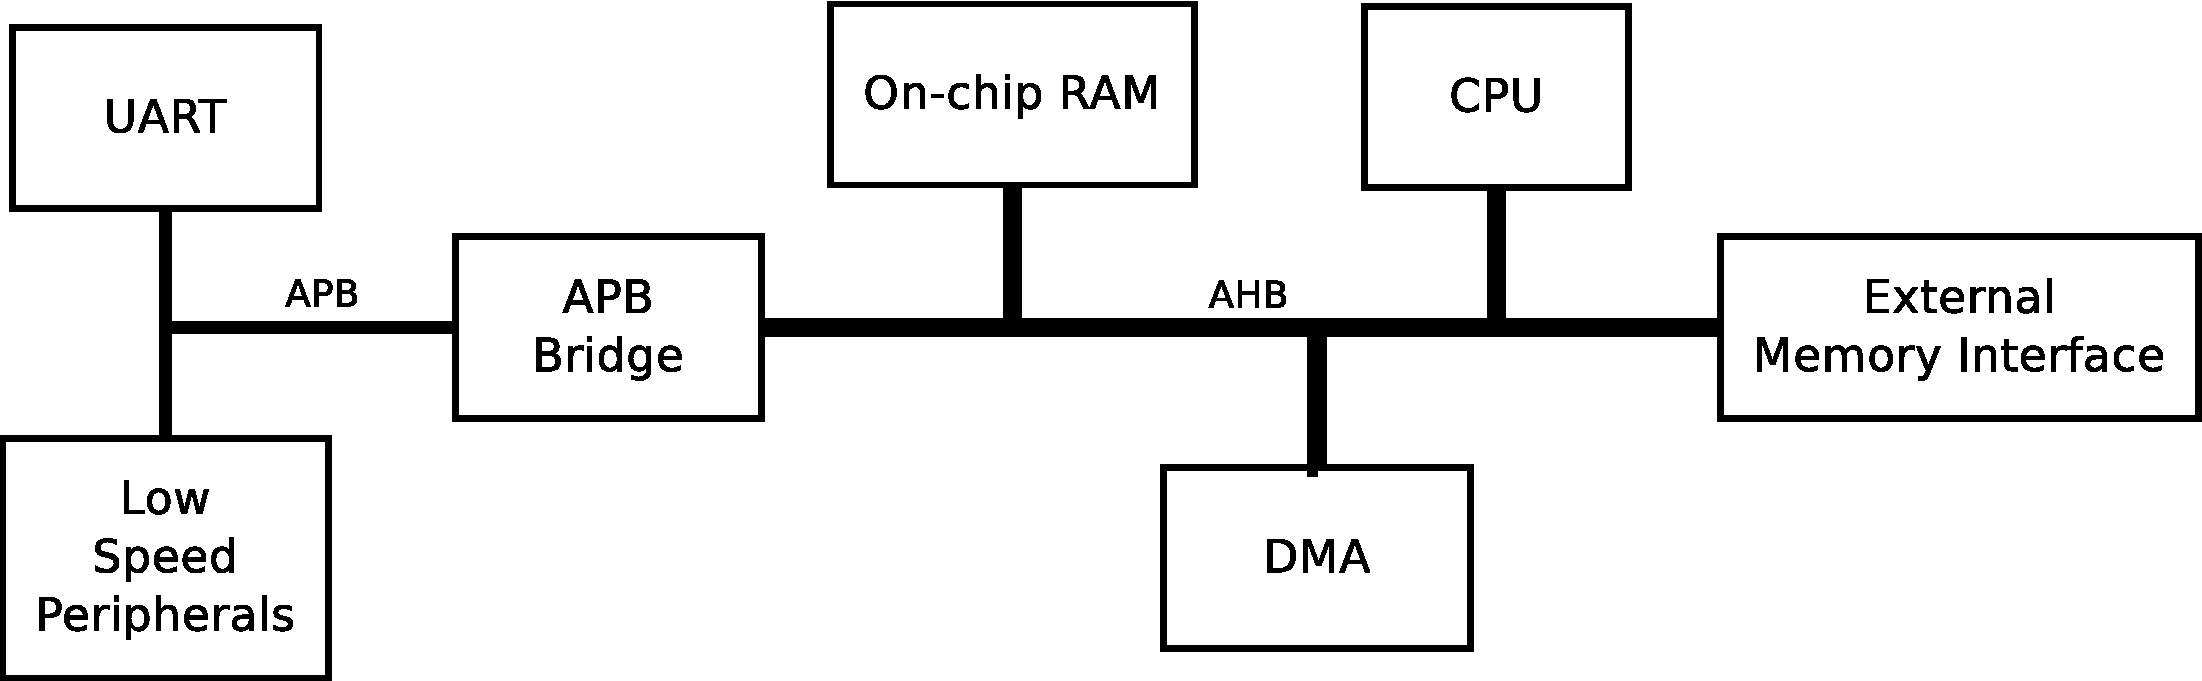
\includegraphics[width=1\textwidth]{figures/pdf/typical_amba_new.pdf}
    \caption{Typical \amba~ system , with a CPU , DMA and other low bandwidth peripherals. }
    \label{fig:general}
\end{figure}

The BUS used in the LEON3 processor is the Advanced High-performance Bus (AHB), where on-chip memory and other peripherals also reside. This bus provides a high-bandwidth interface between the elements connected to it, also, located on the bus is a bridge to the lower bandwidth APB, where most of the peripheral devices in the system are located. Figure \ref{fig:general} exemplify a traditional AHB utilization.

\amba~ AHB implements the features required for high-performance, high clock
frequency systems including:
\begin{itemize}
 \item {burst transfers}
\item {split transactions}
\item {single-cycle bus master handover}
\item {non-tristate implementation}
\item {wider data bus configurations (64/128 bits).}
\end{itemize}

 
\subsection{\amba~ AHB operation}

\begin{figure}[!ht]
    \centering
    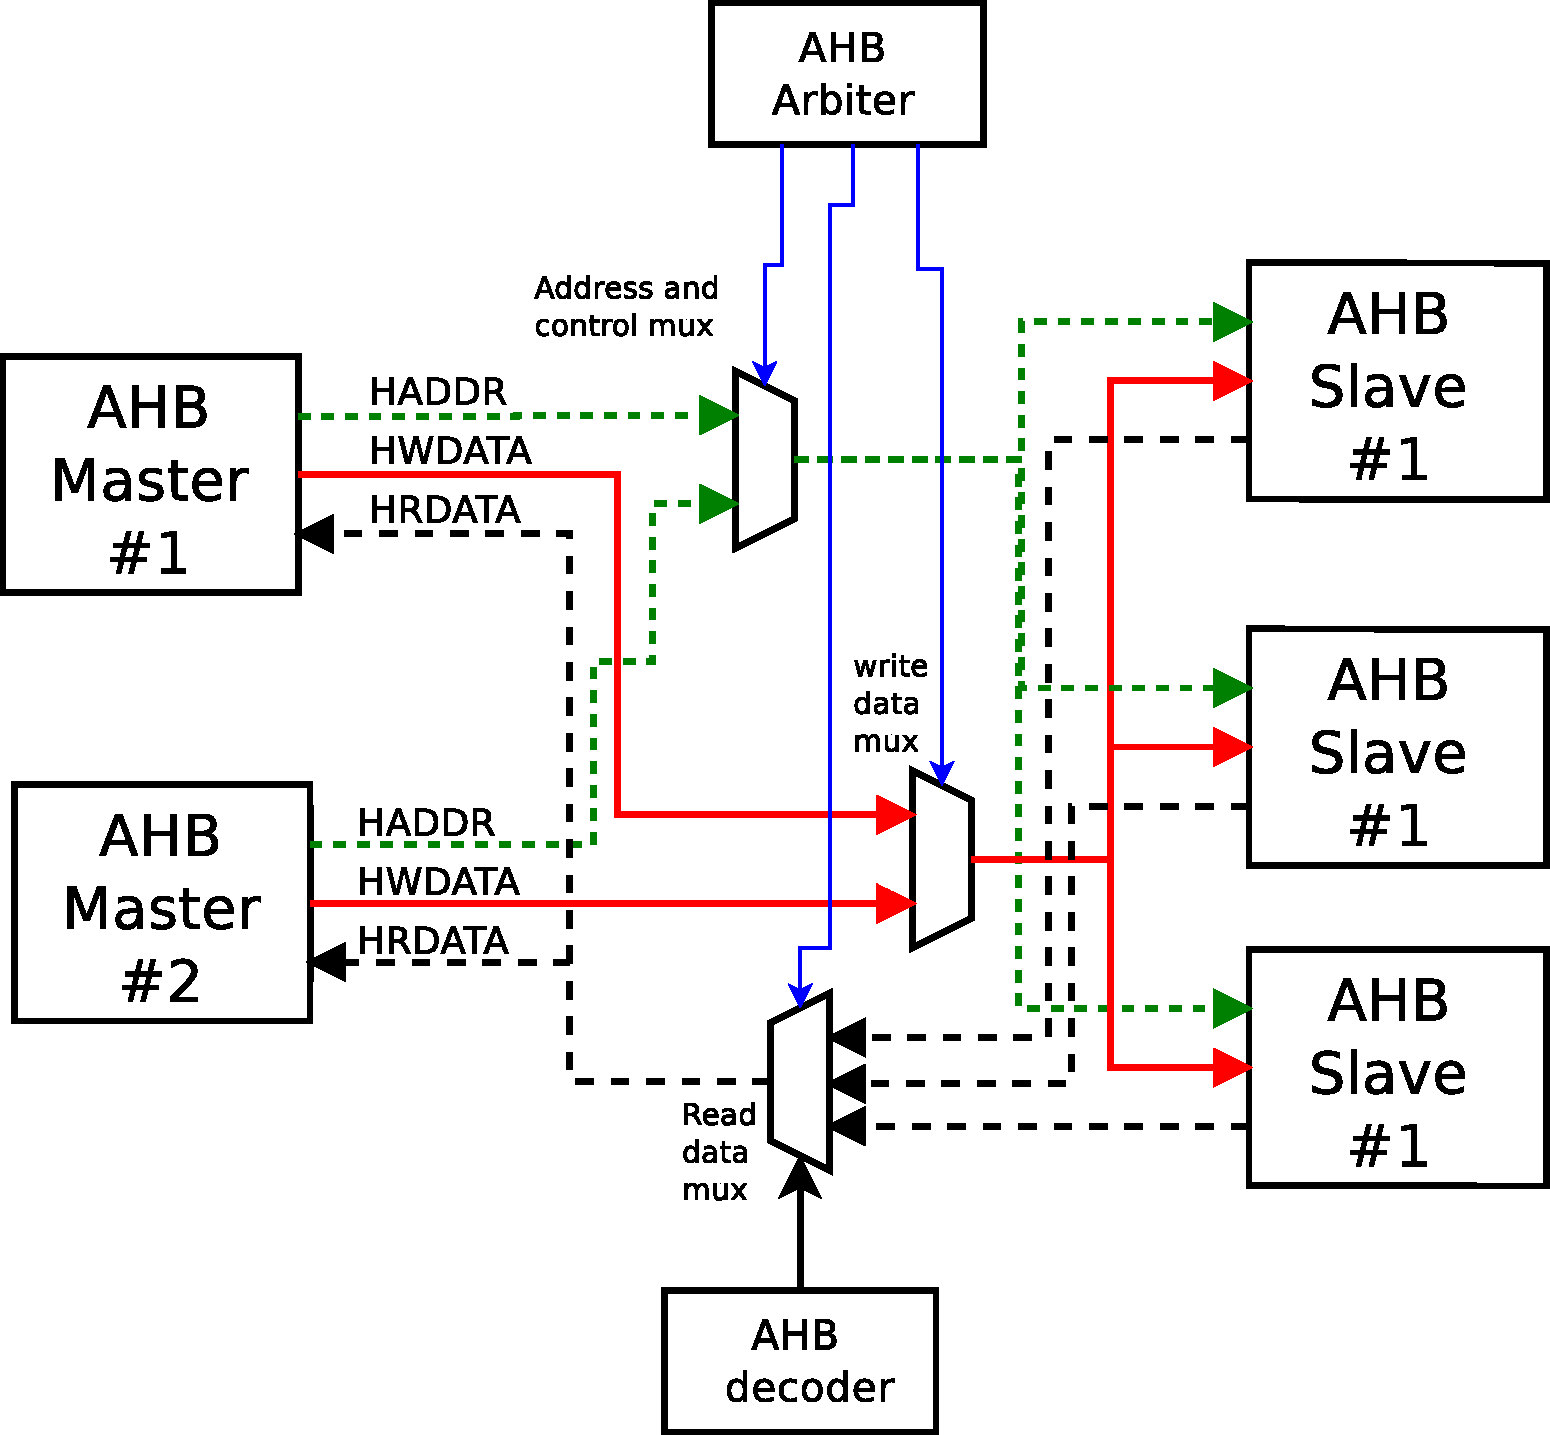
\includegraphics[width=0.7\textwidth]{figures/pdf/amba2_arbiter.pdf}
    \caption{Overview  of the \amba~ Organization, with the arbiters masters and slaves distribution.}
    \label{fig:internorg}
\end{figure}

The previously described \amba~ components are seen by the bus as masters and slaves, as depicted in Figure \ref{fig:internorg}, where, for instance, the CPU is an \amba~ master and the on-chip RAM is a slave. Who decides the priorities and decode all access is the \amba~ arbiter, which will be described further.

Before an \amba~ AHB transfer, from now on just referred to as transfer, can commence the bus master must be granted access to the bus. This process is started by the master asserting a request signal to the arbiter. Then the arbiter indicates when the master will be granted use of the bus. A granted bus master starts a transfer by driving the address and control signals. These signals provide information on the address, direction and width of the transfer, as well as an indication if the transfer forms part of a burst. Two different forms of burst transfers are allowed:
\begin{itemize}
\item incremental bursts, which do not wrap at address boundaries
\item wrapping bursts, which wrap at particular address boundaries.
\end{itemize}

A write data bus is used to move data from a master to a slave, during a read data bus
is used to move data from a slave to a master.
Every transfer consists of:

\begin{itemize}
\item an address and control cycle
\item one or more cycles for the data.
\end{itemize}

\begin{figure}[!ht]
    \centering
    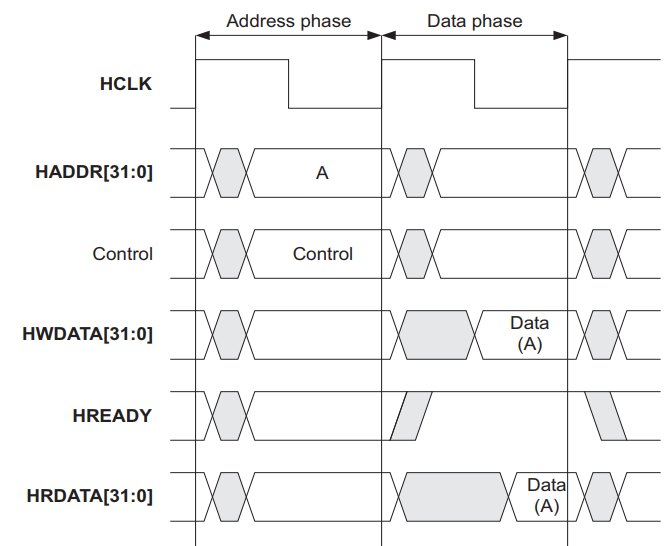
\includegraphics[width=0.4\textwidth]{figures/others/simple_ahb_transfer.png}
    \caption{AHB basic transfer with one cycle for address and control and one or many for data.}
    \label{fig:basic_ahb_transfer}
\end{figure}


In the address and control cycle, the address cannot be extended, and therefore, all slaves must sample the address during this time. The data, however, can be extended using the HREADY signal. When LOW these signal causes wait states to be inserted into the transfer and allow extra time for the slave to provide or sample data, as can be seen in Figure \ref{fig:basic_ahb_transfer}. During a transfer, the slave shows the status using the HRESP response signal where the  following values are used:

\begin{itemize}

\item  {OKAY -} The OKAY response is used to indicate that the transfer is progressing normally and when HREADY goes HIGH this shows the transfer has completed successfully.
\item {ERROR -} The ERROR response indicates that a transfer error has occurred and the transfer has been unsuccessful.
\item {RETRY and SPLIT  -} Both the RETRY and SPLIT transfer responses indicate that the transfer cannot complete immediately, but the bus master should continue to attempt the transfer. In normal operation, a master is allowed to complete all the transfers in a particular burst before the arbiter grants another master access to the bus. However, in order to avoid excessive arbitration latencies, it is possible for the arbiter to break up a burst and in such cases, the master must re-arbitrate for the bus in order to complete the remaining transfers in the burst.
\end{itemize}


\subsection{\amba~ Components}
%\augusto{say that we are reducing the scope to what was used in the design }
These \amba~ components are a  subset of the entire \amba~ features, the focus of this sections is to provide the basis to understand of the signals and work required for the \cshia~implementation, for a full reference please check \cite{ARMAMBA2}.

\subsubsection{Masters}
\begin{figure}[!ht]
    \centering
    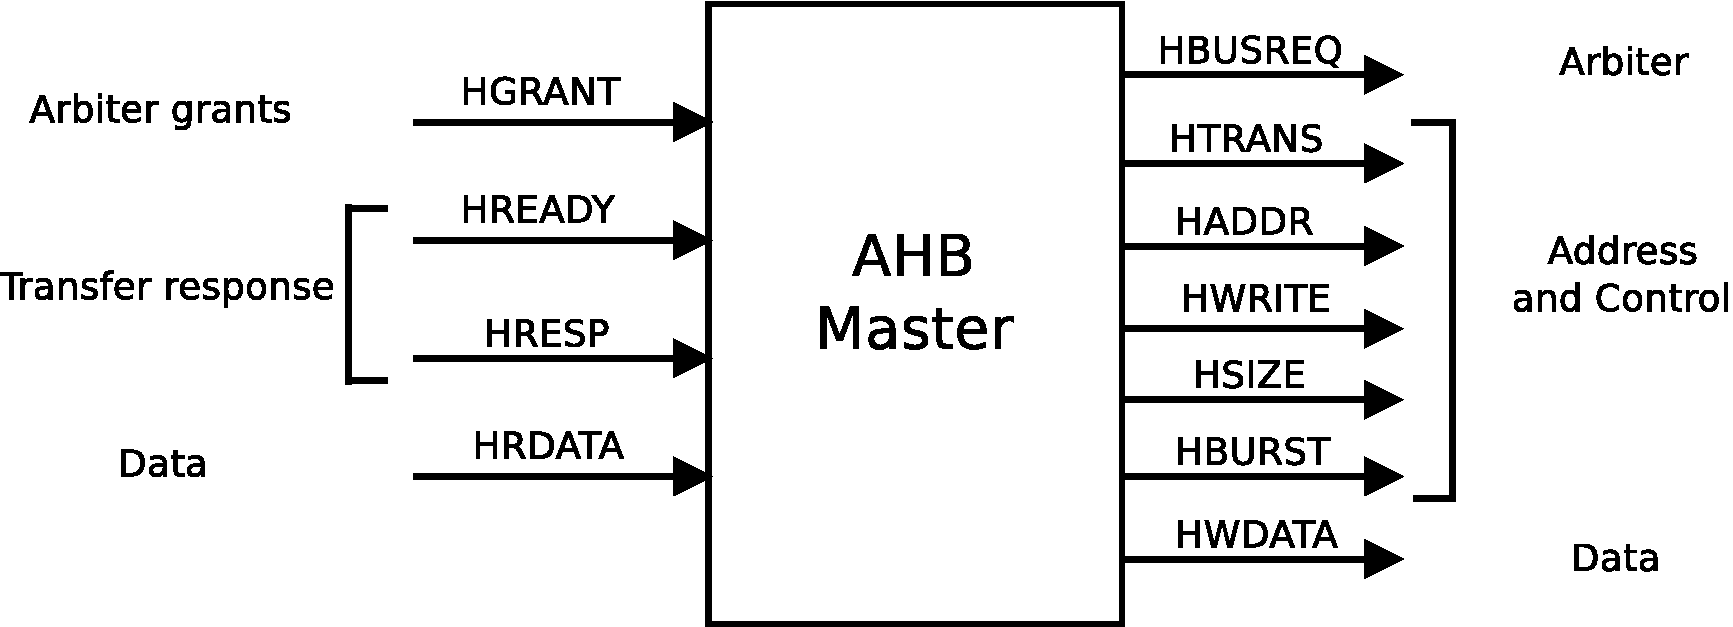
\includegraphics[width=0.7\textwidth]{figures/pdf/ahb_master_new.pdf}
    \caption{AHB master interface, with control and data signals. The HBUSSREQ and HGRANT signals  will be used take control over the bus.}
    \label{fig:masterint}
\end{figure}

 An AHB bus master has the most complex bus interface in an \amba~ system, and these interfaces are depicted in Figure \ref{fig:masterint}. The master contains one direct interface with the arbiter to receive and request the bus grant, a group of control signals to control the flow and duration of the transfer and to interfaces for reading and write data.  Typically an \amba~ system designer would use predesigned bus masters and therefore would not need to be concerned with the detail of the bus master interface.



\subsubsection{Slaves}

\begin{figure}[!ht]
    \centering
    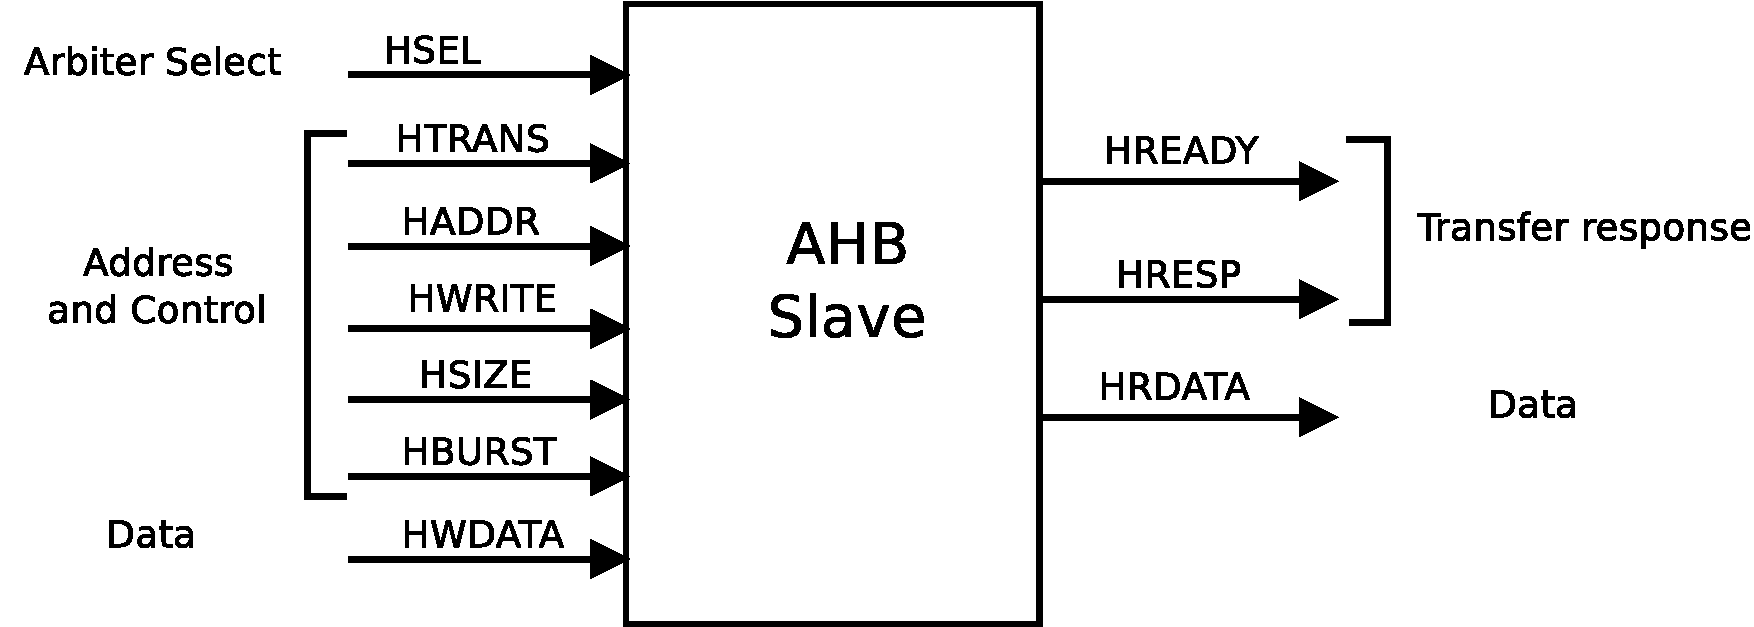
\includegraphics[width=0.7\textwidth]{figures/pdf/ahb_slave_new.pdf}
    \caption{AHB slave interface, where the HSEL signal will indicate when to start transfers.}
    \label{fig:slaveint}
\end{figure}
An AHB bus slave, as depicted in Figure \ref{fig:slaveint}, uses almost the same signals as the master, the difference is that the slave never controls the bus, so,  the interface with the arbiter is being selected as active and respond to transfers initiated by bus masters within the system. The slave uses an HSEL select signal from the decoder to determine when it should respond to a bus transfer. All other signals required for the transfer, such as the address and control information, will be generated by the bus master.
 
\subsubsection{Arbiter}
\begin{figure}[ht]
    \centering
    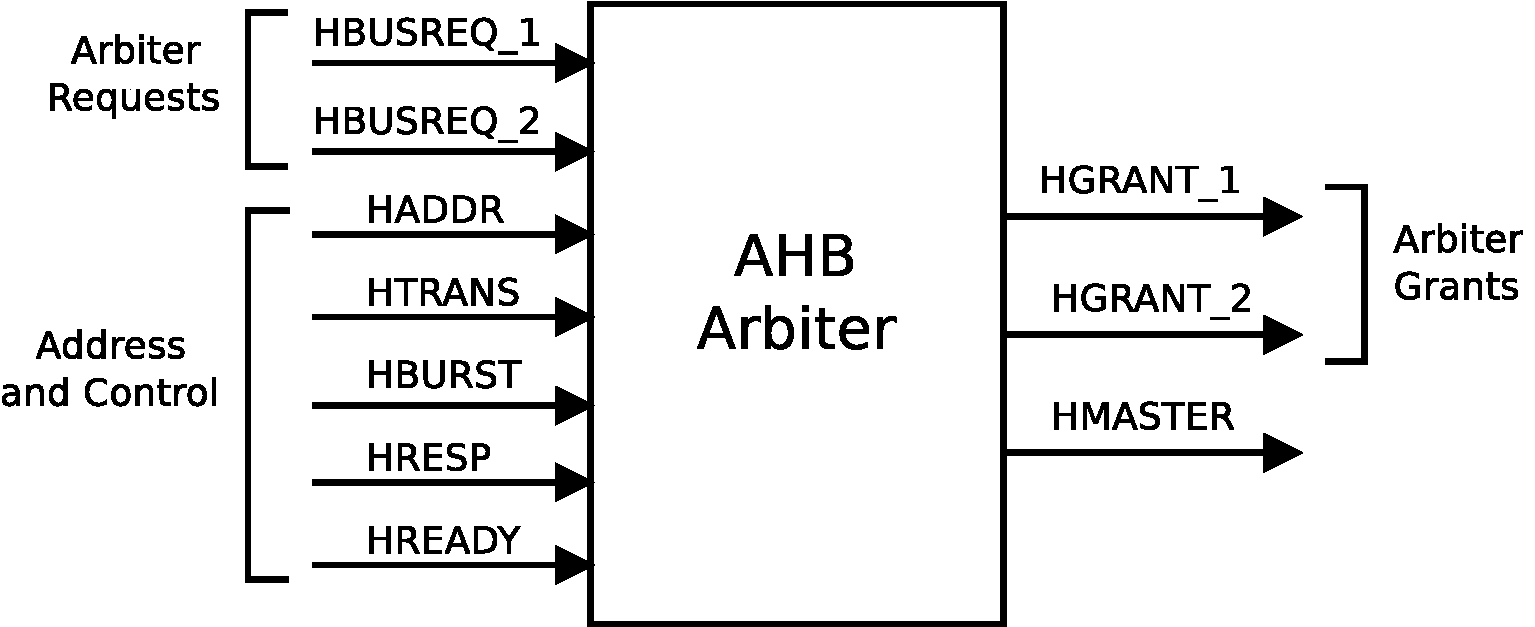
\includegraphics[width=0.7\textwidth]{figures/pdf/ahb_arbiter_new.pdf}
    \caption{AHB arbiter interface with one HGRANT and one HBUSSREQ for each master.}
    \label{fig:arbiterint}
\end{figure}

 The role of the arbiter in an \amba~ system is to control which master has access to the bus. As can be seen in Figure \ref{fig:arbiterint} every bus master has a REQUEST / GRANT interface to the arbiter and the arbiter uses a prioritization scheme to decide which bus master is currently the highest priority master requesting the bus. The detail of the priority scheme is not specified and is defined for each application. It is acceptable for the arbiter to use other signals, either \amba~ or non-\amba~, to influence the priority scheme that is in use.
 The address and control signals are used by the arbiter to route the HWDATA and the HADDR from the granted master to the selected slave as illustrated in Figure     \ref{fig:internorg}.
 
 
 \subsubsection{Arbitration}
 
 The arbitration process needs specific control signals, despite the ones described below, two more signals are used in the \amba~ system, HLOCK and HSPLIT,  the first to indicate that the master wants exclusive access to the bus, the second to restart transactions when they are interrupted.
 
 \begin{itemize}

\item  {HBUSREQ - } The bus request signal is used by a bus master to request access to the bus. Each bus master has an HBUSREQ signal to the arbiter and there can be up to 16 separate bus masters in any system.

%\item  {\textbf{HLOCKx -}} A master asserts the lock signal at the same time as the bus request signal. This indicates to the arbiter that the master is performing many indivisible transfers and the arbiter must not grant any other bus master access to the bus once the first transfer of the locked transfers has commenced. HLOCKx must be asserted at least a cycle before the address to which it refers, in order to prevent the arbiter from changing the grant signals.

\item  {HGRANT - } The grant signal is generated by the arbiter and indicates that the appropriate master is currently the highest priority master requesting the bus, taking into account locked transfers and SPLIT transfers. A master gains ownership of the address bus when HGRANT is HIGH and HREADY is HIGH at the rising edge of HCLK.

\item  {HMASTER - } The arbiter indicates which master is currently granted using the HMASTER signal and,  this same signal can be used to control the central address and control multiplexer, automatically routing the correct HDATA and control signals to the correct slave. The master number is also required by SPLIT-capable slaves so that they can indicate to the arbiter which master can complete a SPLIT transaction.

%\item  {\textbf{HMASTLOCK -}} The arbiter indicates that the current transfer is part of a locked sequence by asserting the HMASTLOCK signal, which has the same timing as the address and control signals.

%\item  {\textbf{HSPLIT[15:0] -}} The 16-bit Split Complete bus is used by a SPLIT-capable slave to indicate which bus master can complete a SPLIT transaction. This information is needed by the arbiter so that it can grant the master access to the bus to complete the transfer.
\end{itemize}

An Example of a master requesting the bus control is shown in Figure \ref{fig:gnwsm} where the arbiter grants the access after a few waiting cycles.
%  \begin{figure}[ht]
%     \centering
%     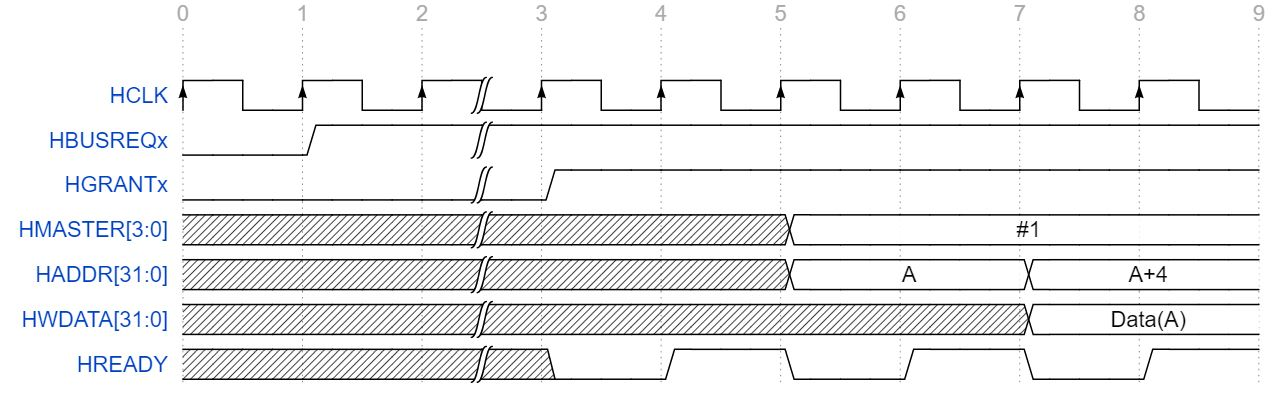
\includegraphics[width=\textwidth]{figures/read_grant_wc_new.JPG}
%     \caption{Granting with wait cycles}
%     \label{fig:grantwait}
% \end{figure}


\subsubsection{Decoder}

\begin{figure}[ht]
    \centering
    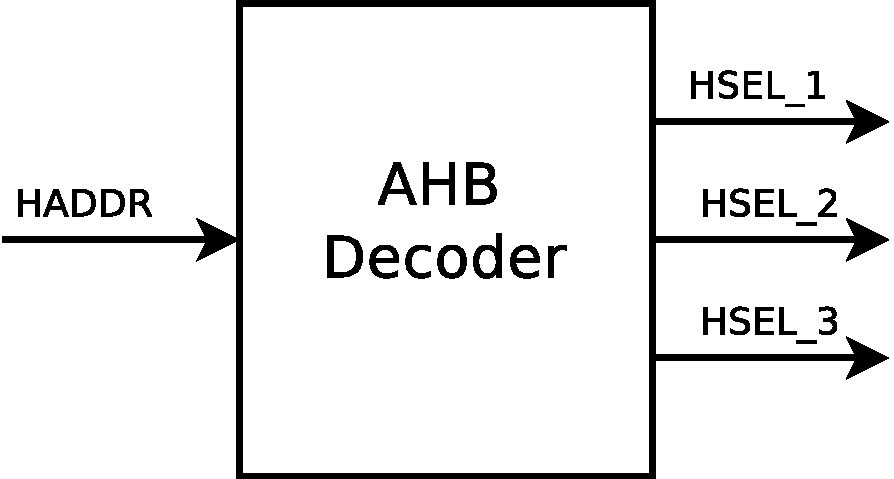
\includegraphics[width=0.6\textwidth]{figures/pdf/ahb_decoder_new.pdf}
    \caption{AHB Decoder interface}
    \label{fig:decoder int}
\end{figure}
 The decoder in an \amba~ system is used to perform a centralized address decoding function, which improves the portability of peripherals, by making them independent of the system memory map. The Idea is that the decoder will snoop the address and select with slave will respond to the transaction, also, as shown in figure \ref{fig:internorg} the decoder will indirectly control a demultiplexer that will route the signals from the correct slave to the granted master.

 

\section{\cshia~Components}
\label{sec:Components-of-the-Architecture}
\mario{Try a top down approach}
As Section \ref{subsec:integrity} discussed, the main resource to provide integrity are tags. Since \cshia~uses \puf-based keys to generate tags, we called them \puf-Tags, or \ptags~for short. \ptags~are the core of \cshia's design. They will be unique for each instance of \cshia~due to the unclonability property of \pufs. That ensures a one-to-one relationship between programs and instances, providing authenticity. To handle \ptags, three main components are added to conventional embedded system architecture. They are: The \ptag~Memory; the Bus Handler (\handler); and the Security Engine (\seceng). Figure \ref{fig:cshia} shows this design and how components communicate between themselves. 

\ptag~Memory is an external memory and has its own buses. This architectural decision gives freedom to designers that can choose bus width, frequency, address space, etc. Because the processor is not aware of any additional component of \cshia, \handler~intercepts data transfers between processor and memory in order to provide them to \seceng~that generates tags. \handler~can also request data ( on behalf of the processor) to main memory so as form complete memory blocks that are necessary to generate \ptags.

\seceng~has three major sub-components. The main one is the \ptag~Generator (\ptaggen), which uses input data whose length is equal to a memory block concatenated with its address to generate \ptags. The \fuzzy~is only used when the system loses its secret key, for instance, after a power cycle. Thus, when the system is powered on, the \fuzzy~will extract the \puf-based key and provide it to \ptaggen. Finally, we have the \ptag~Memory Management Unit (\pmmu). The main functions of the \pmmu~are to store and request \ptags~from the \ptagmem~and also to decode internal addresses of \ptags~to physical addresses of \ptagmem. 


%======================================================
%Bus Handler
%======================================================
\subsection{Bus Handler (\handler)}
\label{subsec:bushandler}
To implement the \cshia~ architecture, all the security operations described in \ref{sec:opmodes} will be performed using a set of words, ideally an entire cache line that the processor might request but that can be multiple cache lines or any other combination necessary to be in the format of the \seceng~ input, this set of words required to calculate the \ptags~ from now on will be referred as \sline.  The \handler~ has three main functions, monitoring the processor request and respond it when necessary, assemble a \sline~  and prevent the processor the execute unsafe or unverified instructions  as well as don't let  it  write in the bus any unsafe operation. In this context any instruction or data requested written by the processor that was not verified by the \seceng~ is considered unsafe.



%======================================================
%Block Diagram
%======================================================
\subsubsection{Block Diagram}

\begin{figure*}[!ht]
    \centering
    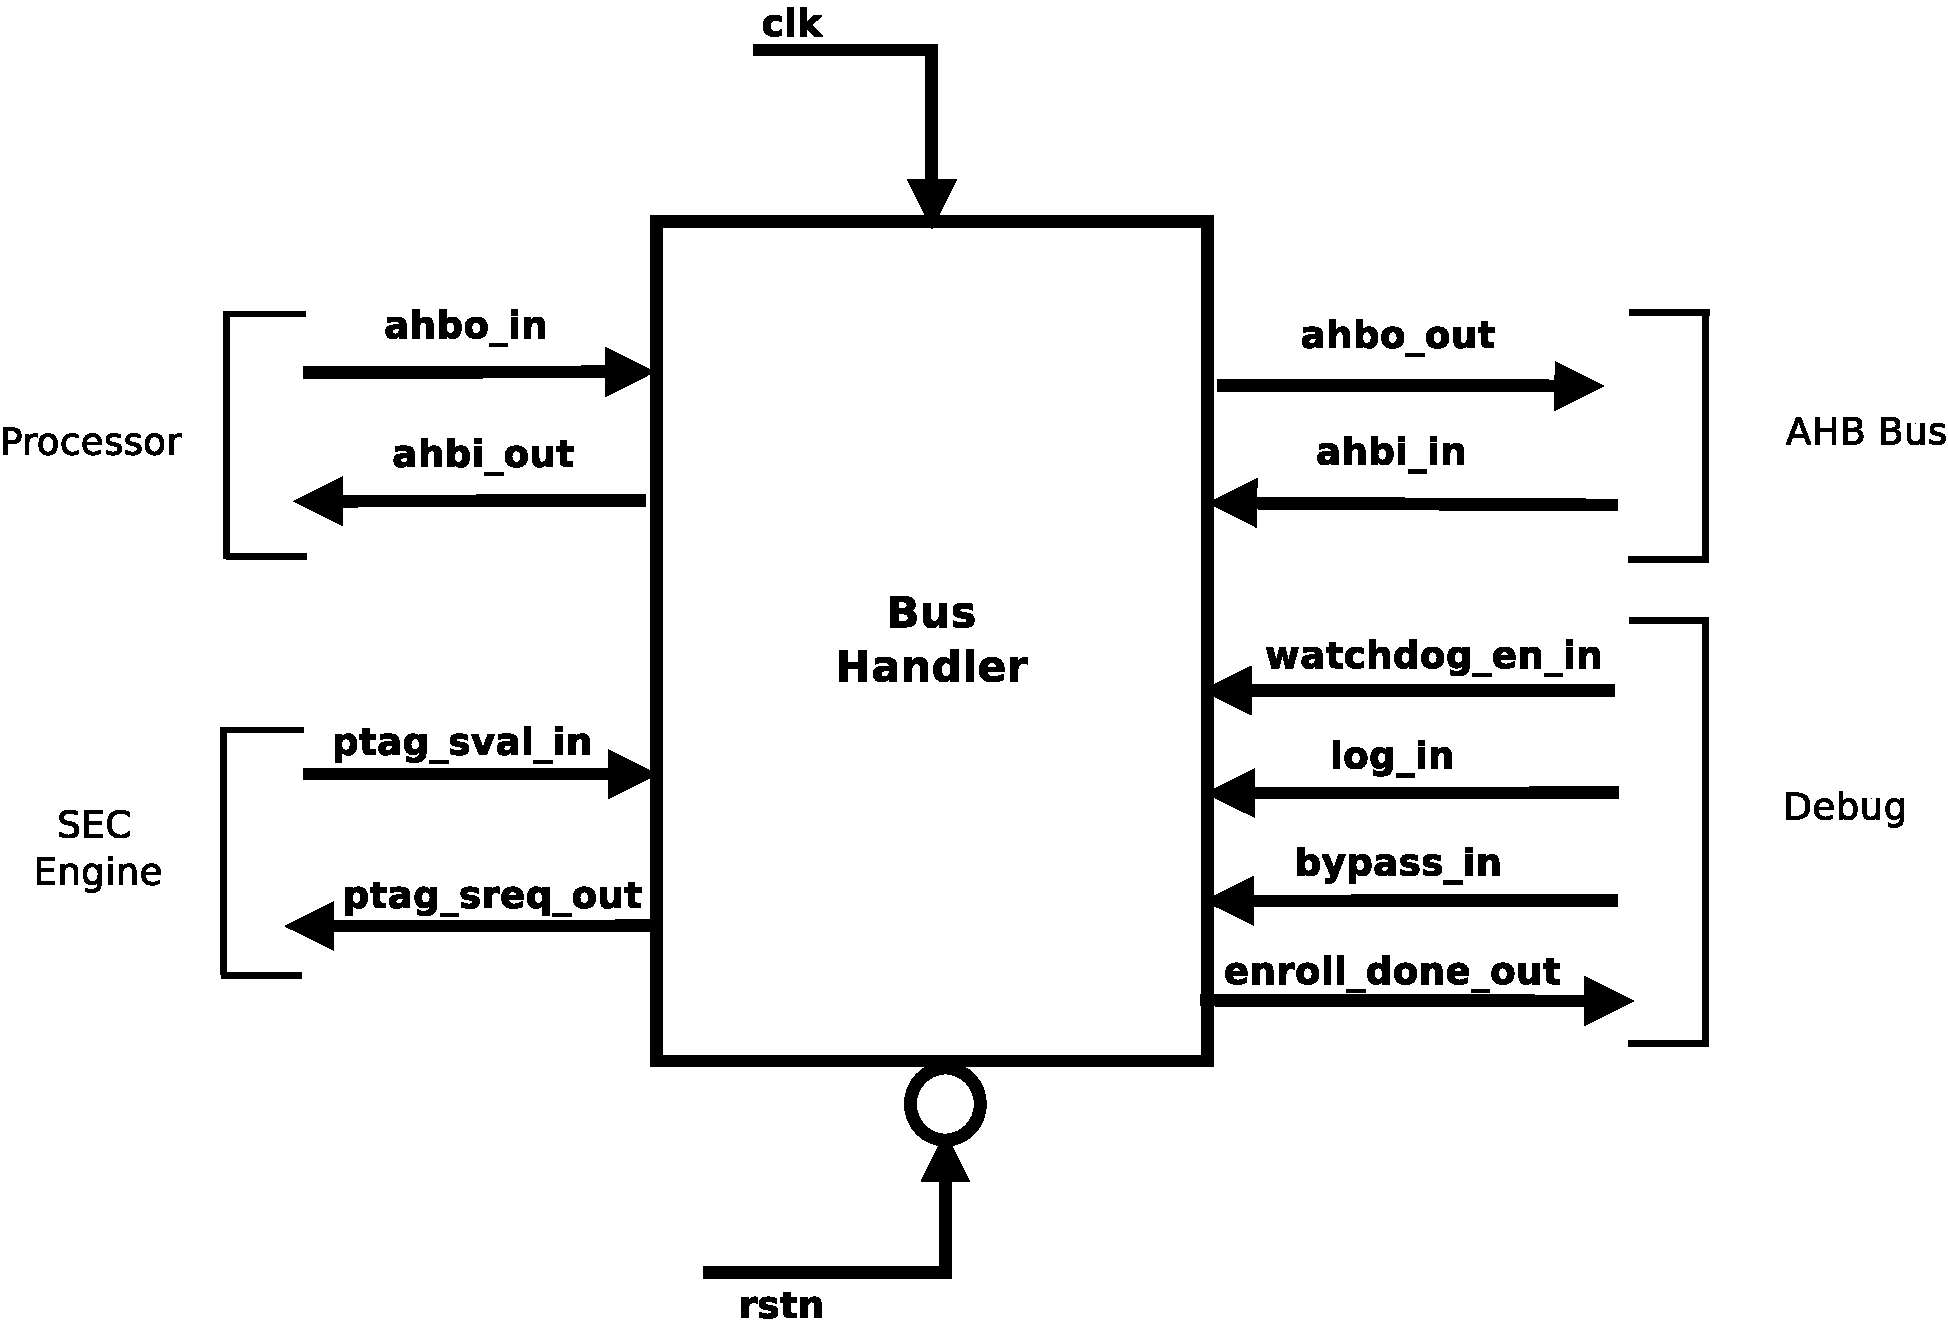
\includegraphics[scale=0.35]{bus_handler}
    \caption{Bus Handler  interface }
%    \vspace*{-9pt} 
    \label{fig:bhbb}
\end{figure*}


%======================================================
%Signal Description
%======================================================
\subsubsection{Signal Description}

The inputs and outputs of this block can be split in four interfaces,
the signals  ahbo\_in and ahbi\_out the interface with the processor,  ahbo\_out  and ahbi\_in
the interface with the bus, ptag\_sval\_in and ptag\_sreq\_out with the security engine and control and debug signals as described in Table \ref{table:shports}.
 The description of each type can be found in Appendix \ref{ap:signals}.

\begin{table}[H]
% \centering
\begin{tabular}{l l l l}
\textbf{Port}   & \textbf{in/out} & \textbf{Type}        & \textbf{Description} 	\\ \hline \hline
clk             & in              & std\_ulogic          & system clock         	\\ \hline
rstn            & in              & std\_logic           & negated rset         	\\ \hline
ptag\_sreq\_out & out             & ptag\_sec\_req\_type & security check request    	\\ \hline
ptag\_sval\_in  & in              & ptag\_sec\_val\_type & security check response  	\\ \hline
ahbi\_in        & in              & ahb\_mst\_in\_type   & AHB input from bus      	\\ \hline
ahbi\_out       & out             & ahb\_mst\_in\_type   & AHB output to processor      \\ \hline
ahbo\_in        & in              & ahb\_mst\_out\_type  & AHB input from processor    \\ \hline
ahbo\_out       & out             & ahb\_mst\_out\_type  & AHB output to BUS            \\ \hline
std\_logic         
bypass\_in      & out             & std\_logic           & bypass input         	\\ \hline
log\_in         & in              & std\_logic           & log bus activities       \\ \hline
watchdog\_en\_in  & in            & std\_logic           & enable a watchdog             \\ \hline
enroll\_done     & out             & std\_logic          & enrollment phase status            \\ \hline

\end{tabular}
 \caption{Description of the \handler~ ports .}
 \label{table:shports}

\end{table}

\subsubsection{Functional Description}

\begin{figure*}[!ht]
	\centering
	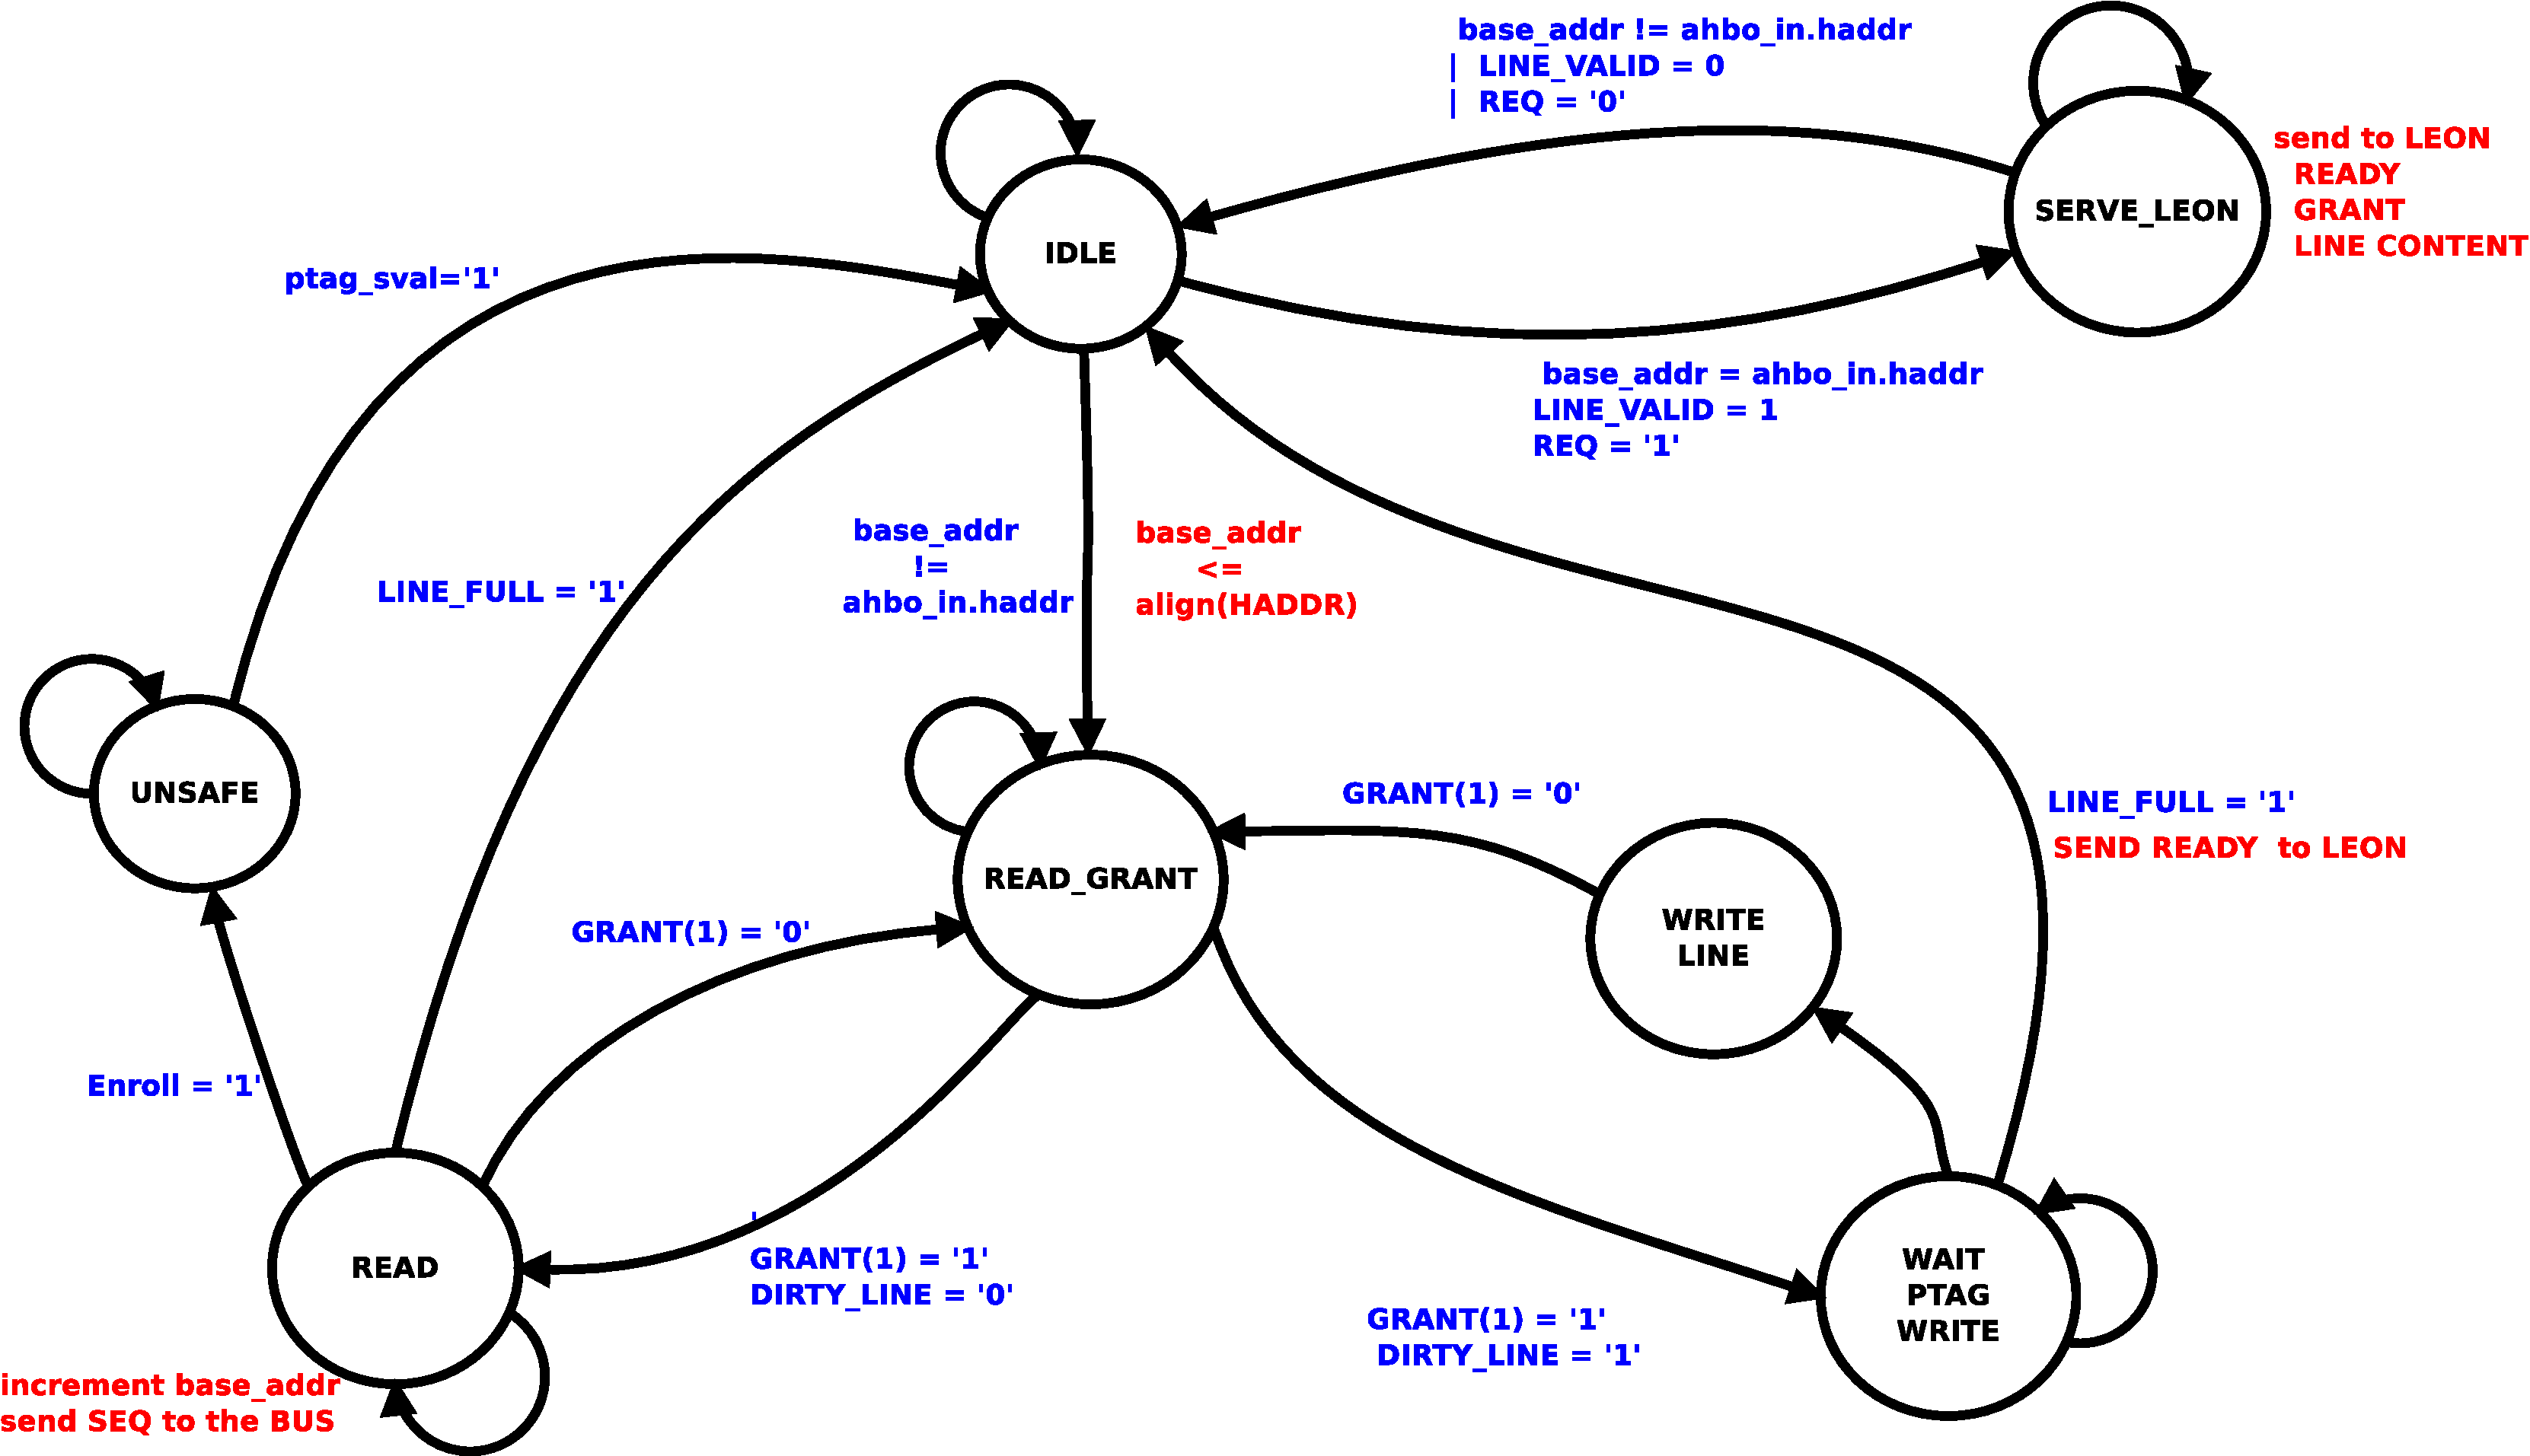
\includegraphics[scale=0.25]{figures/pdf/sec_hand_state_machine.pdf}
    \caption{Bus Handler state machine. The blue text indicate the condition necessary to the transition to happen, the red text indicates the \handler~ actions.   }
%	\vspace*{-9pt} 
	\label{fig:phsm}
\end{figure*}

As shown in Figure \ref{fig:cshia} the processor will see the \handler~ as the bus, and by the bus as the processor, assembling \slines~  and constantly sending those lines to \seceng.  To store the \slines, an internal buffer with a configurable size is used; this is the \handler~ \sline~ buffer and will be from now on referred to as \sbuf.  When the processor requests the bus, the \handler  will assert the grant, and depending on the state of the \sbuf, load new \slines~ from the bus or send one from the \sbuf. The \handler~ is implemented using a state machine which gives the block stability to assemble the \sline~ and to control the flow to the processor and to \seceng. Since this state machine controls all \handler~ operations the functional  description of this block can be explained using the state transitions  of Figure \ref{fig:phsm} and the following state description:

\begin{itemize}
 \item{\textbf{IDLE}}
 
The system stays in this state until the processor asserts HBUSSREQ, at this time the \handler~, on behalf of the arbiter, will answer these requests according to one of these scenarios:
 \begin{enumerate}
     \item The \sbuf~ contains the address requested by the processor in a \sline~ - In this case, the processor can start the transaction in the SERVE LEON state.
     \item The address requested is not in the \sbuf~ - In this scenario, the \handler~ will get the grant in the READ GRANT state and evaluate if its a read or a write, then assemble a new \sline.
     \item The processor requested a line that was not verified or verified incorrectly by \seceng~ -  In this case, the system will halt because a security flaw was detected.
 \end{enumerate}

 
  \item{\textbf{READ GRANT}}

  This state is required for any transaction in the bus, it requests the bus grant for the arbiter, asserting the HBUSSREQ signal on behalf of the processor before beginning the transaction. The arbiter can answer in two possible ways, with or without wait states, for the first, illustrated in Figure \ref{fig:gnwsm},  the HBUSSREQ is asserted in time $2$, by the time the arbiter responds, at time $3$, HGRANT and HREADY are asserted  indicating that the transaction can start in the next cycle. For the second, depicted in figure \ref{fig:gwsm}, The  HBUSSREQ is asserted on time $2$, but the HREADY signal is only asserted on time $5$ delaying the start of the transactions to time $7$, in situations like this the HREADY signal regulates all the traffic. 
  
  
\begin{figure}[!ht]
    \centering
    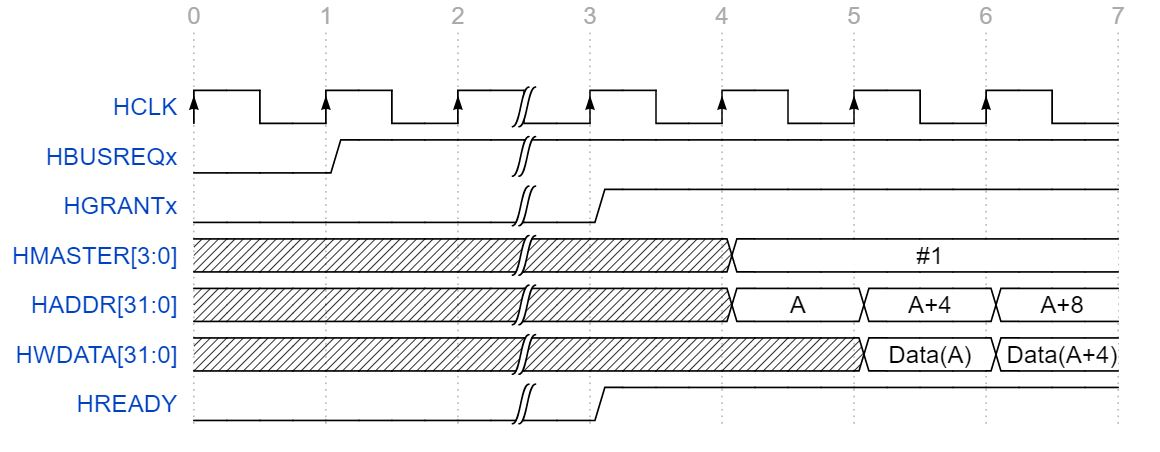
\includegraphics[width=\textwidth]{figures/others/read_grant_no_wait_new.JPG}
    \caption{Requesting grant with no wait states  }
    \label{fig:gnwsm}
\end{figure}


\begin{figure}[!ht]
    \centering
    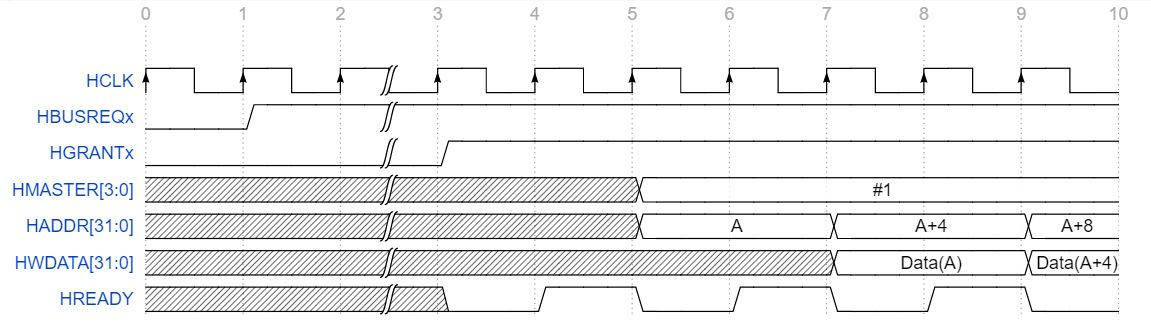
\includegraphics[width=\textwidth]{figures/others/read_grant_ec_new_exended.JPG}
    \caption{Requesting grant with wait states  }
    \label{fig:gwsm}
\end{figure}

  
  Once the arbiter asserts HGRANT,  the \sbuf~ is checked, and one of the positions is selected to be replaced, if the chosen \sline~ contains any updated value by the processor, then it needs to be written in the memory before loading a new \sline. In this is the case, \handler~ will send it to the \seceng~ to calculate a new \ptag~ before writing the line in the memory,  then change to WAIT PTAG WRITE  state while the security operations are done. If no changes were made in the \sline then a new one is loaded in the READ LINE state. 
  
  \item{\textbf{READ LINE}}
  
  A new \sline will be loaded from the main memory into the \sbuf to start a transaction after the bus is granted and all the control signals are in place, as described in section \ref{sec:amba2}. The Figure \ref{fig:ublsm} illustrates two different incremental read transfers,  the first  starts on time $2$ indicated by the first HTRANS=NONSEQ, with  halfword size reading positions $0$x$20$ and $0$x$22$, the second transaction starts at time $4$ where a small delay is exemplified to show how the HREADY controls the bus operations, and then three words are transferred to the master.  Once an entire \sline is transferred, the line is sent to \seceng~ and the state is set to IDLE again, where the system will halt until the execution is considered secure.
  After a power cycle, all the instructions are read and tagged, in this case, the execution is not safe, so the state is set to UNSAFE before going back to IDLE. This process is explained in Section \ref{sec:opmodes}.

  
 
  \begin{figure}[!ht]
    \centering
    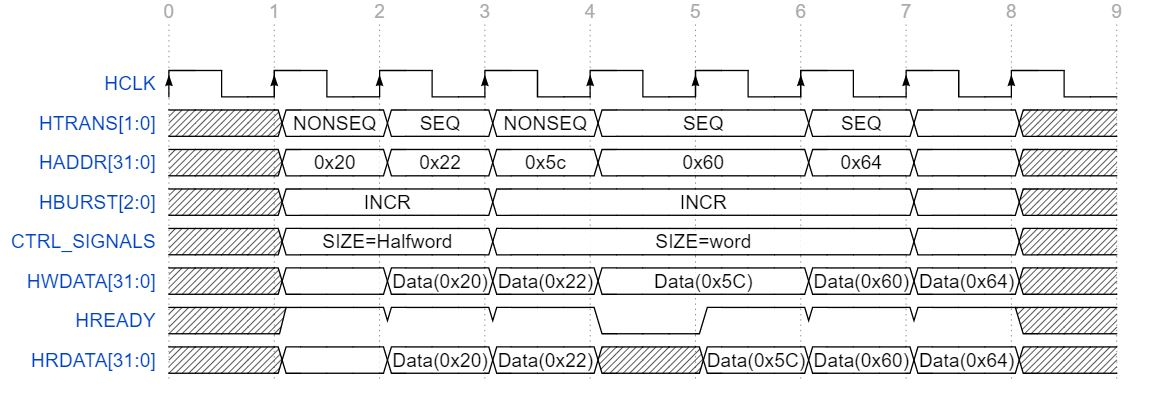
\includegraphics[width=\textwidth]{figures/others/basic_transfer_w_ctrl_new.JPG}
    \caption{Incremental burst transfers with halfword and word.}
    \label{fig:ublsm}
  \end{figure}
  
 \item{\textbf{WAIT PTAG WRITE}}
 When a \sline need to be written, first is sent to the \seceng~ to calculate the respective \ptag~ and store in the \ptagmem, this process can take a different number of cycles depending on the features used in the \seceng~, this process is explained in Section \ref{sec:secengine}. After the \ptag is calculated the line can be written in the state WRITE LINE.
 
 
 \item{\textbf{WRITE LINE}}
   \begin{figure}[H]
    \centering
    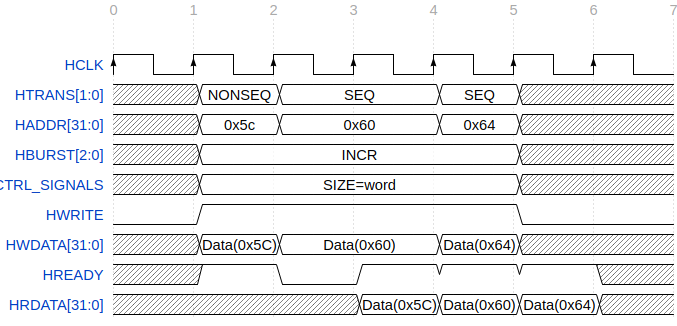
\includegraphics[width=\textwidth]{figures/others/ahbwrite.png}
    \caption{Incremental write burst of words.}
    \label{fig:ahbwrite}
  \end{figure}
The write process is much similar to the read, as Figure \ref{fig:ahbwrite} shows the difference is the HWRITE signal that is asserted during the entire transfer. After the write is completed the state is set to IDLE and the \handler~ is ready to send respond the processor requests.

 \item{\textbf{SERVE LEON}}

 On this state all LEON requests read or write are executed, the \handler~~will assert the HGRANT and starting acting like the bus until there is data in the \sbuf. The transfers towards the processor are the same as described before in Figures \ref{fig:ublsm} and \ref{fig:ahbwrite}, when the processor requests any address that is not on the \sbuf, the state is set to IDLE.
 
\item{\textbf{UNSAFE}}
After a power cycle all the instructions are read and tagged in a process called enrollment that can take a different number of cycles depending on the features used in the \seceng~, the enrollment is explained in Section \ref{sec:opmodes}. After a \sline is considered secure during the enrollment phase, the state goes to IDLE.
 
\end{itemize}

%======================================================
%Security Engine
%======================================================
\subsection{Security Engine}
\label{sec:secengine}

\begin{figure*}[!ht]
    \centering
    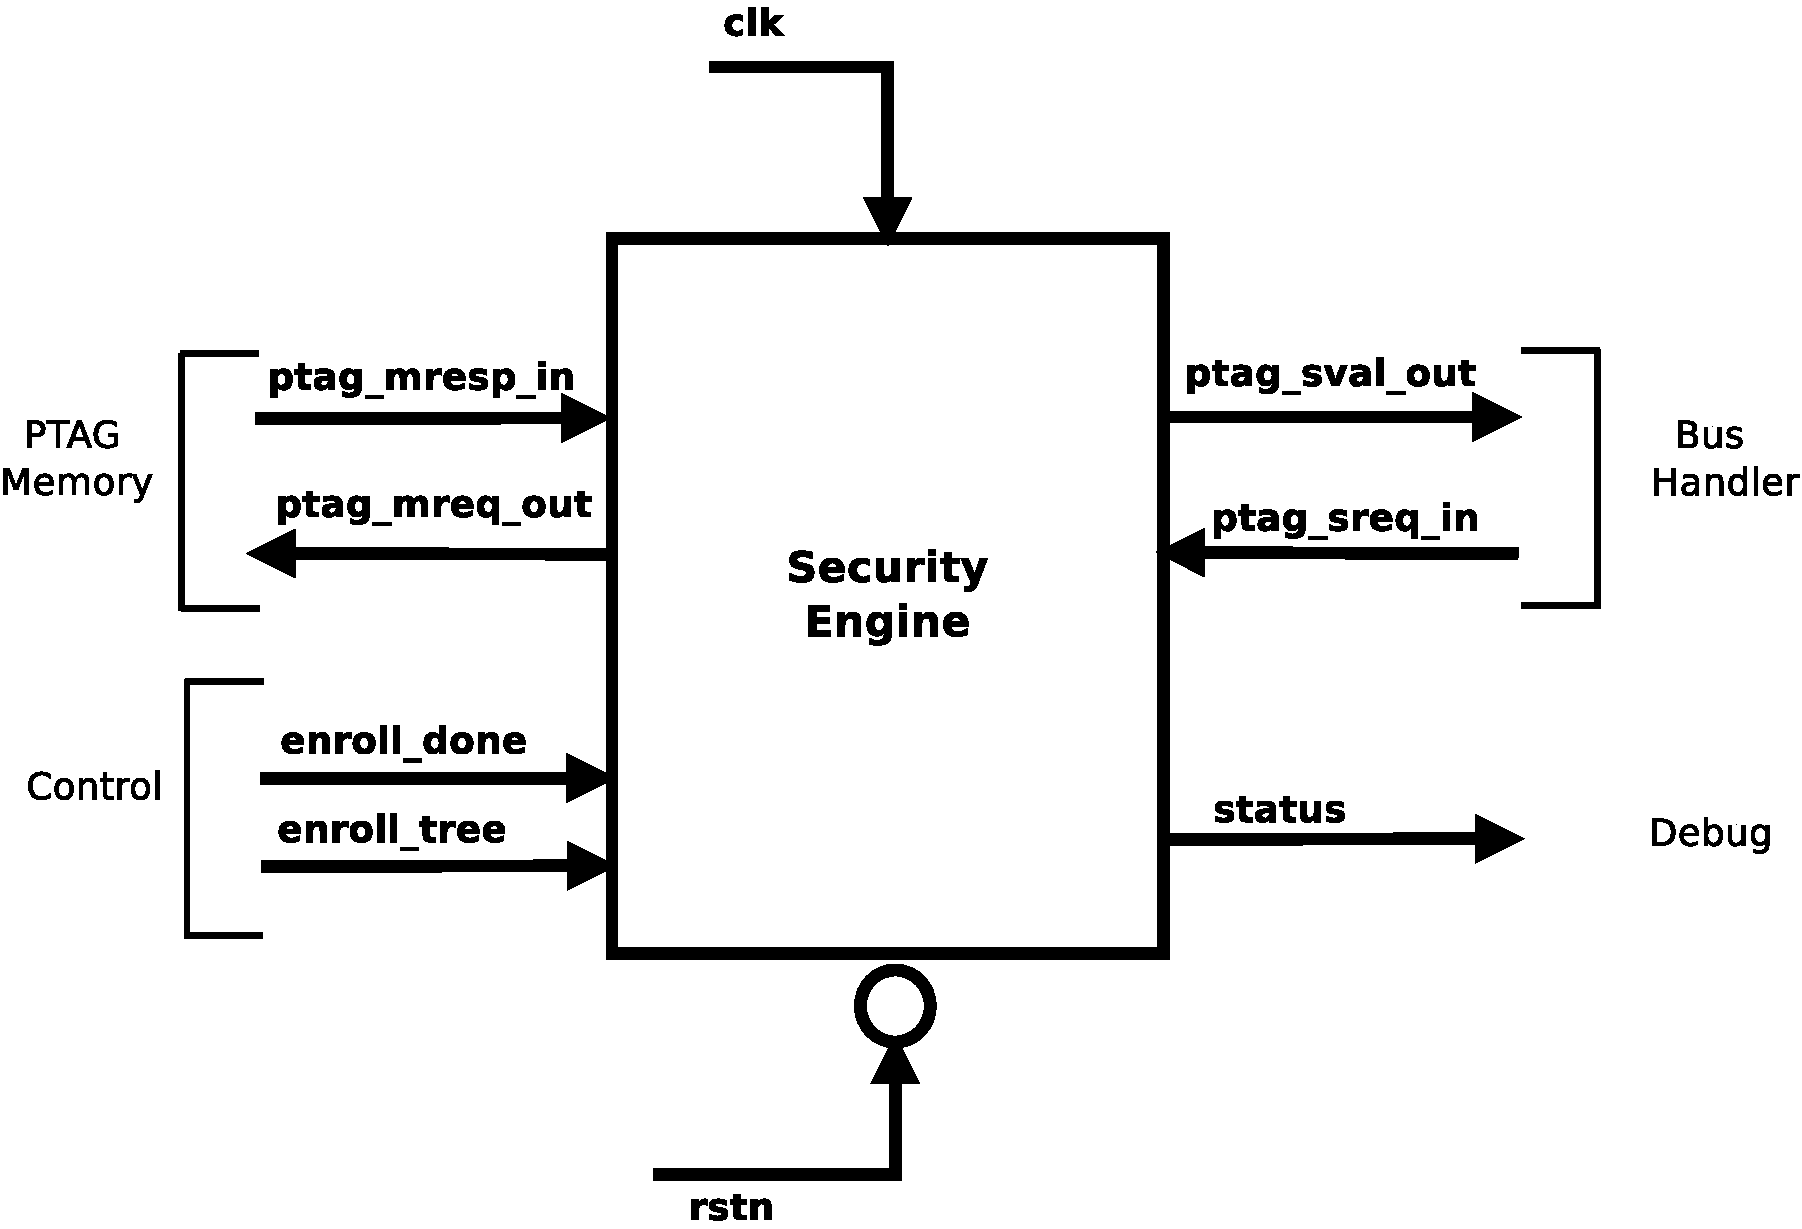
\includegraphics[scale=0.35]{security_engine_bb}
    \caption{Security engine interface.  }
%    \vspace*{-9pt} 
    \label{fig:sebb}
\end{figure*}


This block is responsible for the security part of \cshia~,  as shown in Figure \ref{fig:sebb} it contains one interface toward the \ptagmem~ to read and write \ptags~, one interface towards the \handler~  and also control and debug signals described in Table \ref{table:seports}.  The \seceng~ has three main functions, extract the key from the \puf~, generate and validate \ptags~ and make the \ptagmem operations transparent to \handler~ and the processor.



\subsubsection{Signal Description}
%TODO remove the enroll tree
\begin{table}[H]
    \centering
    \begin{tabular}{l l l l}
    
        \textbf{Port}   & \textbf{in/out} & \textbf{Type}        & \textbf{Description} 	\\ \hline \hline
        clk             & in              & std\_ulogic          & system clock         	\\ \hline
        rstn            & in              & std\_logic           & negated reset         	\\ \hline
        ptag\_sreq\_in  & in              & ptag\_sec\_req\_type & security check request    	\\ \hline
        ptag\_sval\_out & out             & ptag\_sec\_val\_type & security check response  	\\ \hline
        ptag\_mreq\_out & out             & ptag\_mreq\_type 	 & ptag memory  request    	\\ \hline
        ptag\_mresp\_in & in              & ptag\_mresp\_type 	 & ptag memory  response  	\\ \hline
        enroll\_done    & in              &  std\_logic      	 & enroll phase status  	\\ \hline
        %enroll\_tree    & in              &  std\_logic      	 & \mt~control 	\\ \hline
        status          & in              &  std\_logic      	 & internal state 	\\ \hline
        
    \end{tabular}
    \caption{Description of the \seceng~ ports.}
    \label{table:seports}
\end{table}




\subsubsection{Functional Description}

\begin{figure}[!ht]
    \centering
    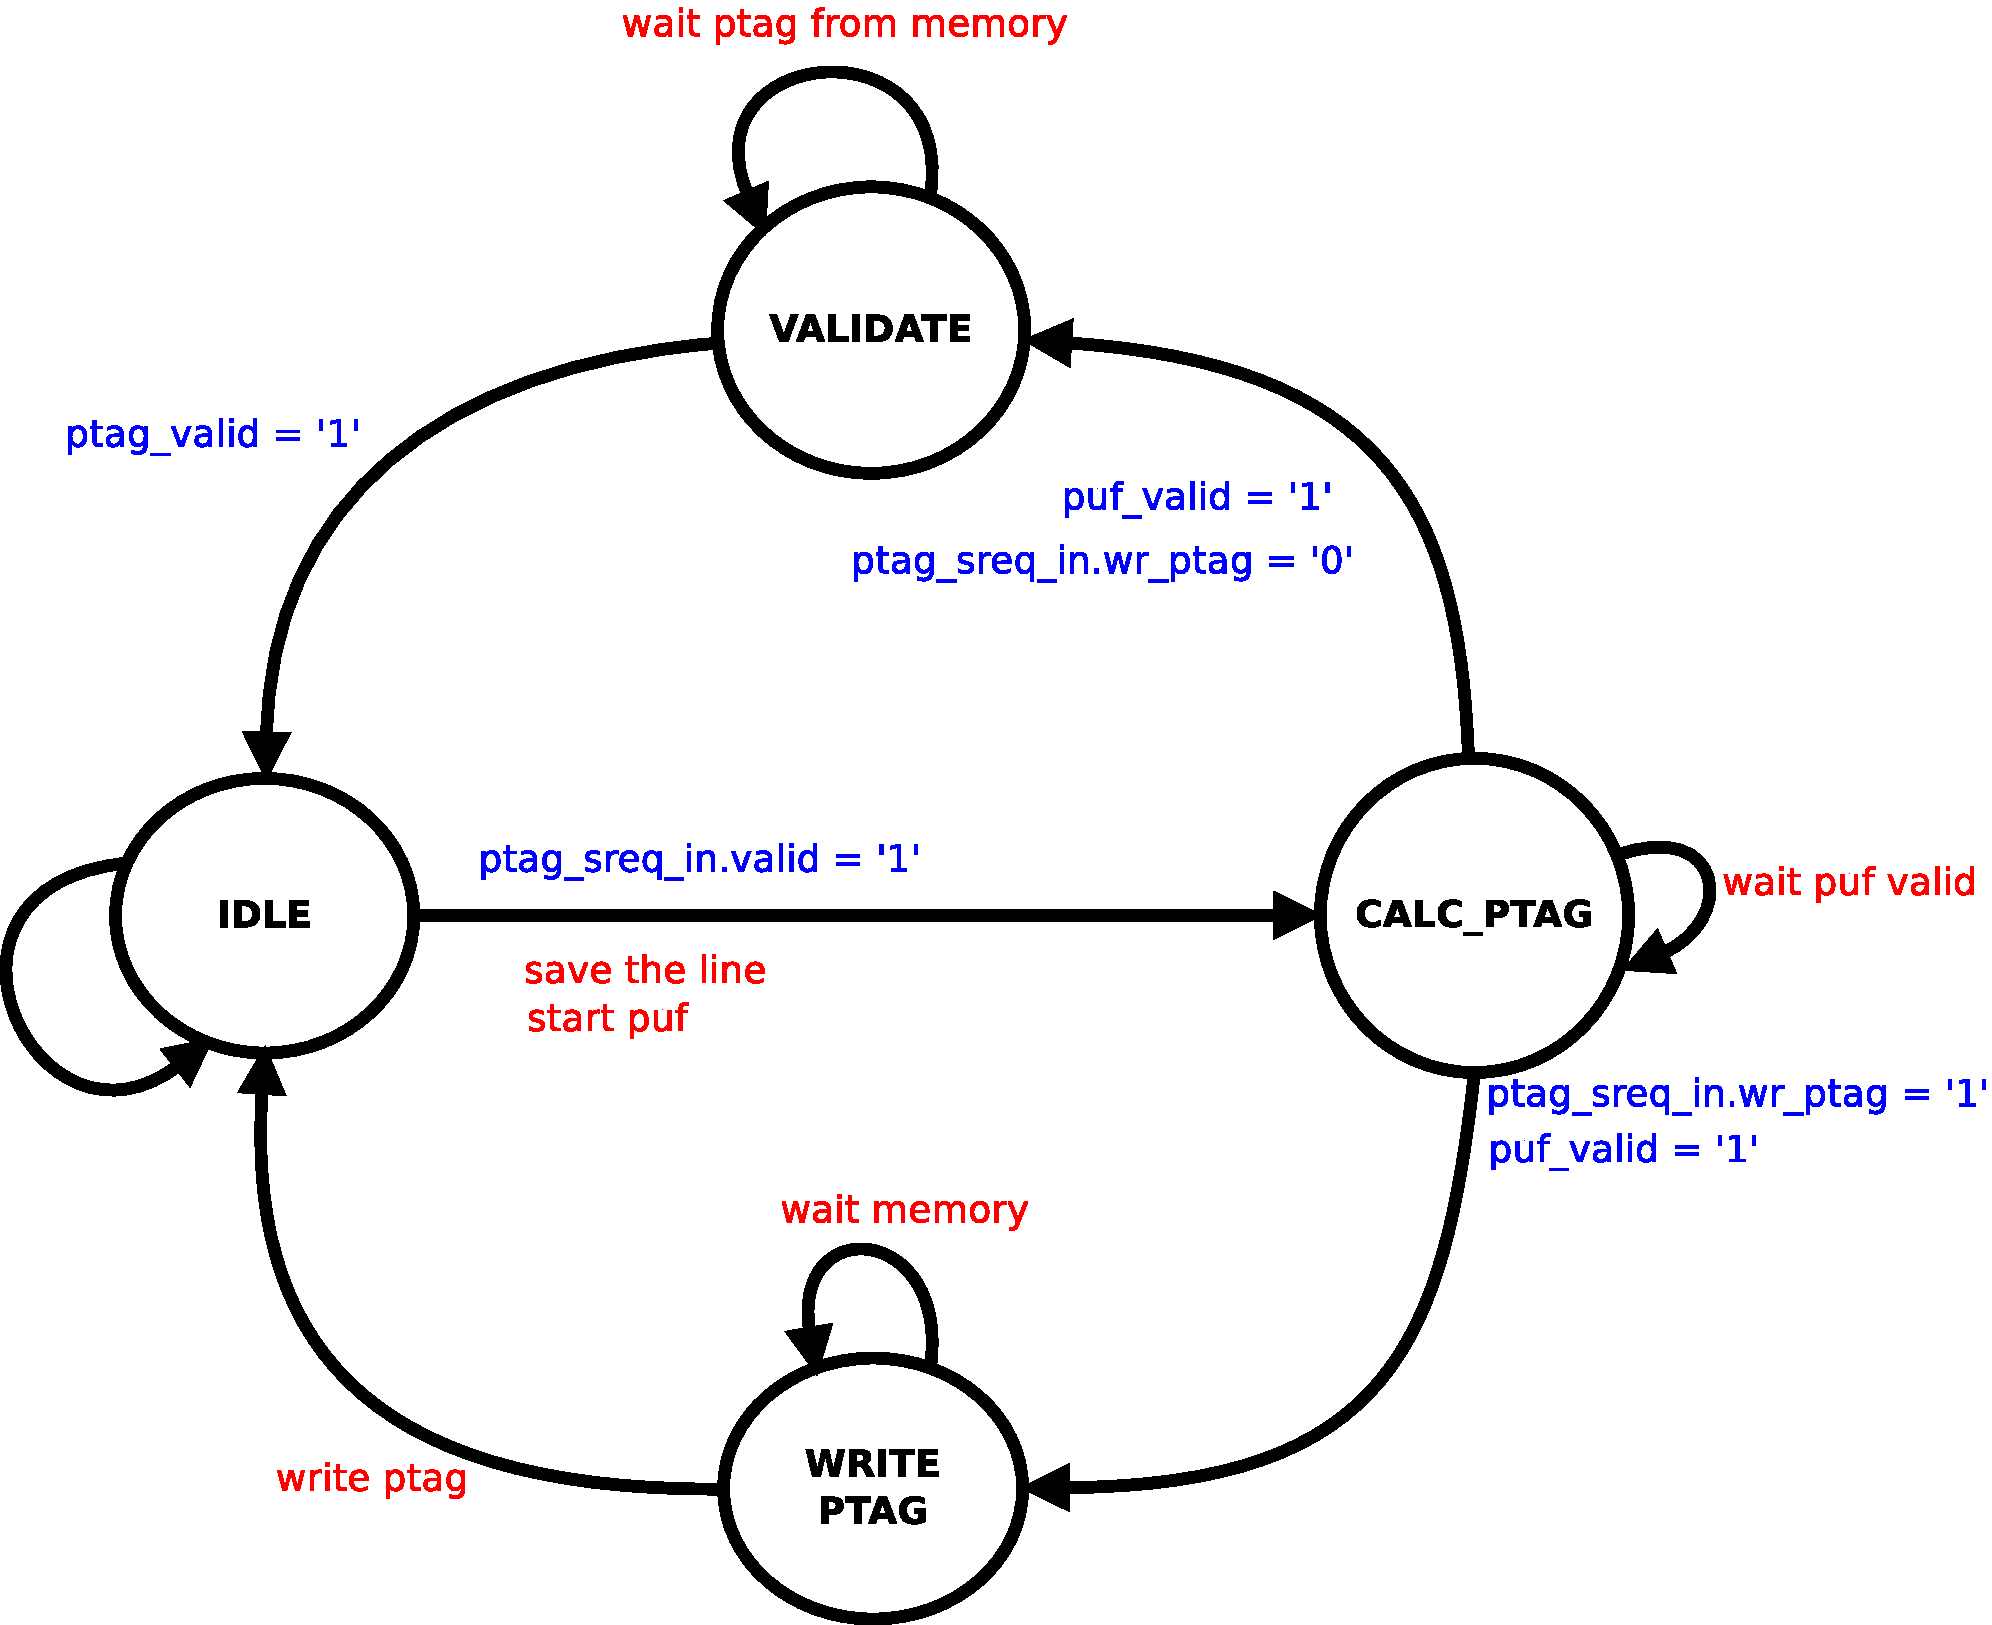
\includegraphics[width=0.70\textwidth]{figures/pdf/sec_engine_sm_no_tree.pdf}
    \caption{\seceng~ state  machine. }
    \label{fig:sesm}
\end{figure}

The \seceng~ is the core of \cshia~, here all the security features take place. This block has the following features: 
\begin{enumerate}
    \item Extract the cryptographic key from the SPUF
    \item Create the \ptags~for each \sline
    \item Validate \ptags an inform the \handler~that the execution is secure
    \item Control the \ptagmem~ 
\end{enumerate}
%TODO remove the tree from the thesis
%There are two possible configurations for the \seceng~, with or without a \mt~ to provide integrity, both options are evaluated in Section \ref{sec:hardware_setup}.
 The implementation of \seceng~ uses a state machine illustrated in Figure \ref{fig:sesm} to synchronize the internal components. The state machine transactions will be used to explain how \seceng~ works.


\begin{itemize}
  \item{\textbf{IDLE}}
 
The \seceng ~ stays in the IDLE  state until a valid \sline~ is sent by the \handler~ when the line arrives either is to write or validate a \ptag~, for both cases, the line will be registered and a \ptag~will be generated, so the next state will be CALC PTAG. 
 
  \item{\textbf{CALC PTAG}}
  After a \sline~ is registered in IDLE state it is used to generate a \ptag, a process that can take many clock cycles. After the \ptag is ready, the initial controls signal from the \handler~ are evaluated and the state is set to either VALIDATE or  WRITE PTAG if this is a write operation. If the next state is  VALIDATE, a request is made to the \pmmu~ to fetch the previously calculated \ptag ~ of the equivalent \sline.
  

  \item{\textbf{VALIDATE}}
  Since in this state the \ptag~ from the \ptagmem and the newly generated one from the CALC PTAG state are ready, the comparison between the two values can be done and the result as a security response to the \handler~ can be sent. Then the system goes back to IDLE.
  

 \item{\textbf{WRITE PTAG}}
  This state signalizes to the \pmmu~  that the \ptag~ from the CALC PTAG state can be written in the \ptagmem~ and confirmation to the \handler~ is sent.
\end{itemize}


\subsubsection{\seceng~ operation }
The\seceng~ operations described in the previous sections can be better visualized as a continuous operation, for this the validate and the write transactions are described next.
\begin{itemize}
 \item{\textbf{Validate \ptag~ - }} As can be seen in Figure \ref{fig:ptgag_rd_no_mt}  on time $2$ the \handler~ sends a  \sline to the \seceng~, the line is registered and the generation of the \ptag~ starts, when the ptag\_ready signal is asserted,  the equivalent \ptag~ for the \sline~ is requested from the \ptagmem~. On time $4$ in one cycle the comparison is made and if the \ptags~ match a line\_secure flag is asserted and the \handler can continue to serve the processor.
 
   \begin{figure}[!ht]
    \centering
    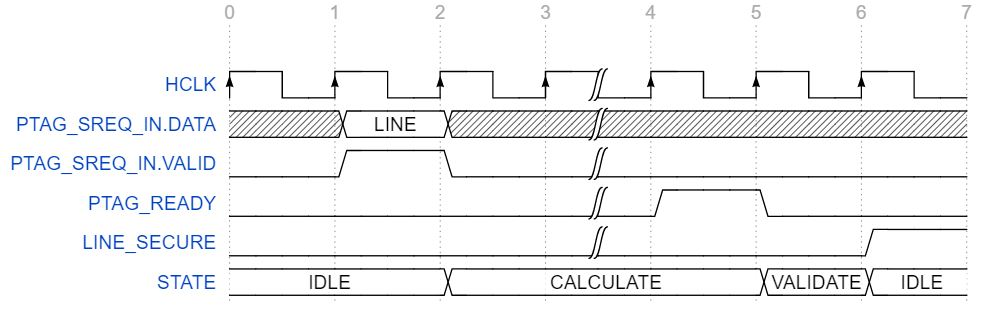
\includegraphics[width=\textwidth]{figures/others/ptag_read_sec_eng.JPG}
    \caption{\ptag~ read and validate on \seceng.}
    \label{fig:ptgag_rd_no_mt}
\end{figure}


 \item{\textbf{Write \ptag~ - }} for a write operation, like in the example from  Figure \ref{fig:ptgag_rd_no_mt}, the \sline~ that  come from \handler~  on time $2$ together with a write request are registered on IDLE state.  Next a new \ptag~ is generated in the CALC PTAG state, after the \ptag~is ready and the ptag\_ready signal is asserted on time $5$, a request to the \pmmu~ is made  to write the new \ptag in the \ptagmem on time $6$, finally the state is back to IDLE  and a line\_secure flag is asserted on time $9$ so the \handler~ can continue its operation. 
   \begin{figure}[!ht]
    \centering
    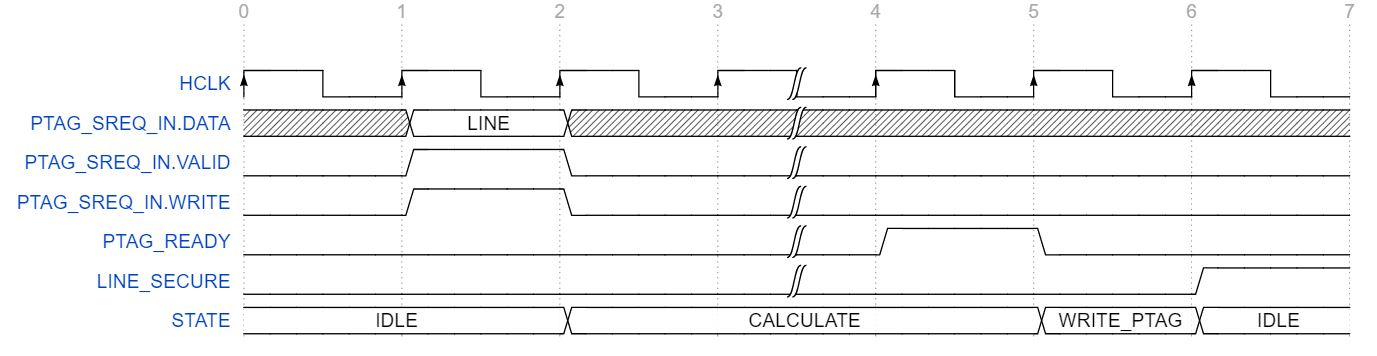
\includegraphics[width=\textwidth]{figures/others/ptag_write_sec_eng.JPG}
    \caption{\ptag~ write  on \seceng.}
    \label{fig:se_pw_no_mt}
\end{figure}
\end{itemize}

%  \begin{figure}[H]
%    \centering
%    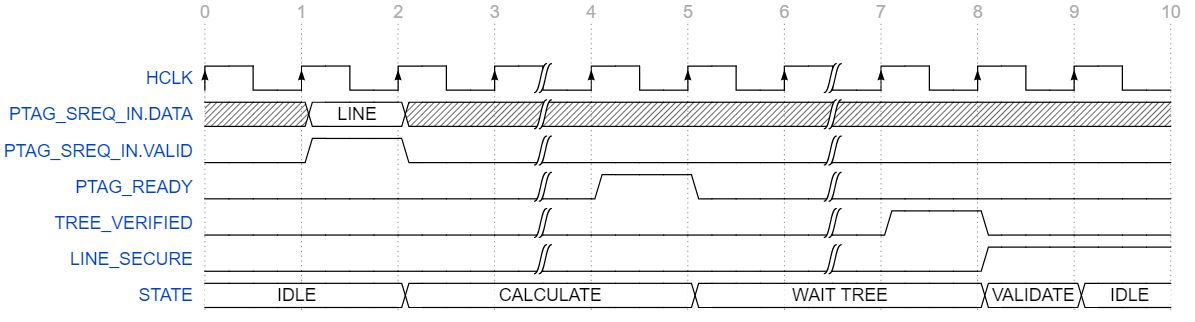
\includegraphics[width=\textwidth]{figures/ptag_read_tree_sec_eng.JPG}
%    \caption{\ptag~ read with \mt }
%    \label{fig:ptgag_rd_mt}
%\end{figure}
%  \begin{figure}[H]
%    \centering
%    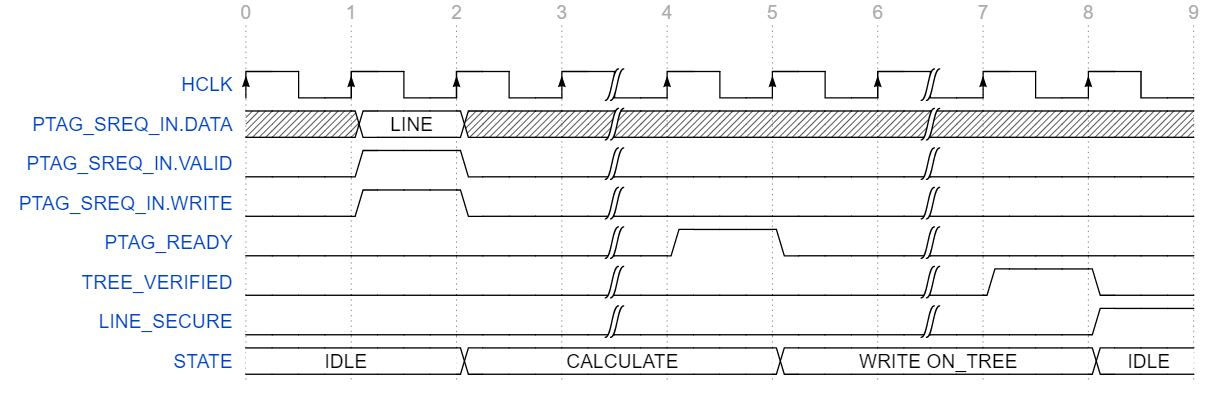
\includegraphics[width=\textwidth]{figures/ptag_write_tree_sec_eng.JPG}
%    \caption{\ptag~ write  on sec engine with \mt.  }
%    \label{fig:se_pw_mt}
%\end{figure}
%===========================================================================================================================================================




\subsection{\ptag~ Memory Management Unit (\pmmu)}
\label{subsec:pmmu}
The main functions of the \pmmu~are to store and request \ptags~from the \ptagmem~ and also to decode internal addresses of \ptags~to physical addresses of \ptagmem. This block is required every time the \handler~ needs to execute a security check, it needs to provide the \ptag ~ from the equivalent \slines~  to be compared in the VALIDATE state of the \seceng~  and write the newly generated \ptags when requested in the WRITE PTAG state of the \seceng.  Other blocks of \cshia~ are agnostic to the \pmmu operation since it controls the \ptagmem~ that is not connected to the bus.
 %In addition to that, \pmmu~can have two distinct designs. 
%If a designer chooses to use timestamps as the solution for replay attacks, \pmmu~will have an internal memory to store and control timestamps of the memory blocks.
% However, if the solution for replay attacks is a \mt\cite{Elbaz2009}, \pmmu~will control verification and update of the tree, as well as it will have cache memory, the \ptagcache, to speed up these tasks.
%\subsubsection{\ptagmem}
%\label{subsubsec:ptagmem}
%\augusto{describe memories connected to  PMMU}


\section{Operation Modes}
\label{sec:opmodes}

%describe all


\subsection{Runtime Phase}
\label{subsec:runtimephase}
\def\fenroll{Figure \ref{fig:fuzzy-extractor} \subref{fig:fuzzy-enroll}}
\def\fregen{Figure \ref{fig:fuzzy-extractor} \subref{fig:fuzzy-regen}}
After the enrollment phase, \cshia~instances are ready for distribution. Here is how \cshia's components work together. \handler~checks for memory read-write operations of the processor. When it perceives a memory read, it will capture memory words \andor~request memory words to compose a memory block. Then it sends this memory block and its address to \seceng. On its turn, \seceng~uses \pmmu~to bring the corresponding \ptag~of that memory block from \ptagmem, while \ptaggen~computes a \ptag~using the content served by \handler. After that, the \ptag~brought from \ptagmem~and the one computed are compared. If they match, \seceng~knows that neither the \ptag~nor the memory block were tampered with. Otherwise, \seceng~alerts the handler that can isolate the processor or sends a non-maskable interrupt to the processor.


For write operations, the process is more straightforward. Once any memory block that reached the processor was verified for integrity and authenticity, \handler~can serve the cache line to \seceng~that uses \ptaggen~to compute a new \ptag~and \pmmu~sends that \ptag~to \ptagmem.  During the product lifetime, the device can be rebooted and turned off and on multiple times. While this will not affect \ptags, which are externally stored in \ptagmem, the secret key has to be recovered every time the system comes back from off-line periods. This recovery procedure of the \fuzzy~is described next.

\subsubsection{Key Regeneration}
\label{subsubsec:Key-Regenation}
\begin{figure}[!t]
    \centering
    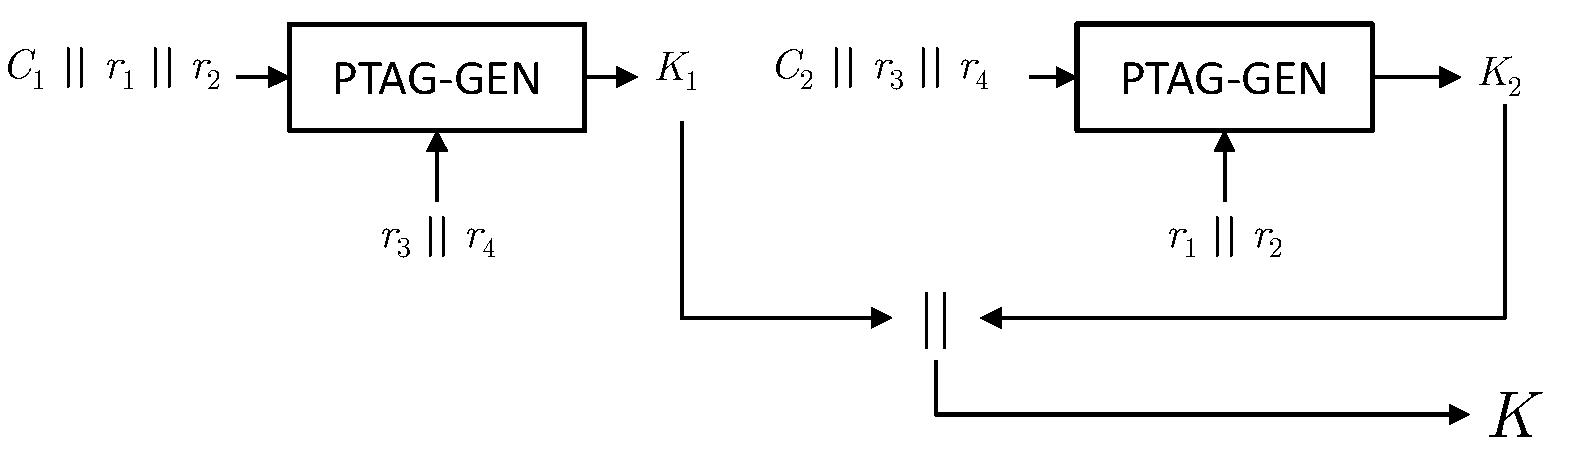
\includegraphics[width=0.7\textwidth]{key-construction}
%     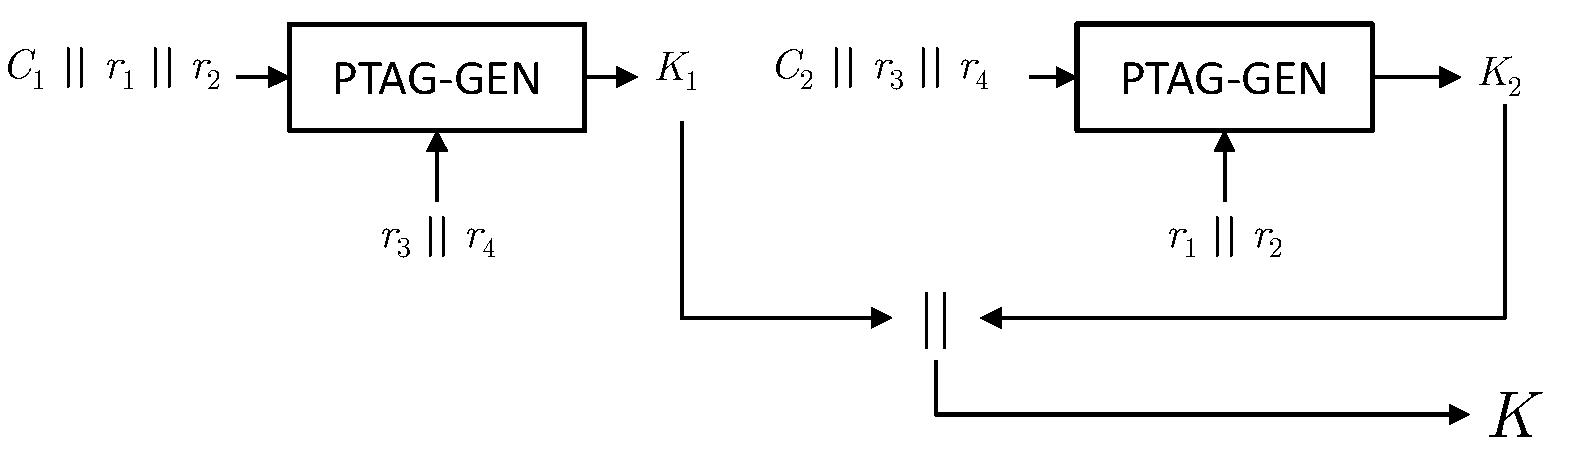
\includegraphics[scale=0.325]{key-construction}
    \caption{Key generation on \cshia.}
    \label{fig:key-construction}
\end{figure}

During the enrollment, there were eight challenges selected to produce four $r_i$ and four $w_i$ values. These challenges and helper data can be exposed off-chip and stored in \ptag~Memory if the designer chooses to do so. The recovery process of the secret key can be seen in \fregen. After using the challenges and all helper data, the syndromes are recovered. Due to inconsistent nature of \pufs, the fuzzy extractor actually recovers bit-flipped versions $w'_i$ and $r'_i$, what leads to the \bch~decoder receive $r'$ and $s'$. Once bit flips in $r_i$ values are corrected, the \fe~uses all $r_i$ to regenerate the secret key as Figure \ref{fig:key-construction} shows.

\subsection{Enrollment Phase}
\label{subsec:Enrollment-Phase}

In order to ensure authenticity and integrity, an initial procedure has to be conducted by the manufacturer\slash{}vendor. This enrollment procedure will activate the \fuzzy~to to extract the secret key from \pufs. Once that is done, the \handler~brings all memory blocks for tag generation. Next, this procedure is explained in detail.

\subsubsection{Key Extraction}
\label{subsubsec:Key-Extraction}

\ptag~Generator implements a Pseudo-Random Function (\prf), which is a primitive cryptographic very similar to a hash function with a significant difference: the input processing is based on a secret key. In order to provide uniqueness to every \cshia~ instance this key has to be unique. As aforementioned, \pufs~cannot be cloned, thus they can provide this uniqueness. Nevertheless, one big conundrum of using electronic \pufs~to generate keys is that they are inherently unstable. Due to their nature of leveraging on the imperfection of the fabrication process, external factors such as temperature variation, voltage variation, etc., can interfere with their responses. Thus, varying responses to challenges during the lifetime of devices. In order to provide consistency in \puf~responses, \fuzzy~(\fe) are employed. In simple terms, \fes~are schemes comprised of an extraction algorithm and a recovery procedure. Becker provides a solid review and formal definitions in \cite{Becker2017:RobustFuzzyExtractor}.

There are multiple ways of implementing a \fuzzy. Originally, \cshia~was proposed using a Code-offset \fe, which is well-known to reduce the entropy of extracted keys \cite{Armknecht2011:Formalization}. To strengthen the \cshia~design, we now use an adapted version of the Index-based Syndrome (\ibs) \fe~proposed by Yu and Devadas in \cite{Yu2010:RobustErrorCorrection}. \fenroll~illustrates the process of key extraction of \cshia's \fe. In general terms, a bit string $r$ is extracted from \pufs. Then, the \fe~generates a syndrome $s$ of $r$ using a $(n,k,t)$ Error Correction Code (\ecc). The \fe~also extracts a bit string $w$ and combines it to the syndrome $s$ to generate an encoded helper data $h$. This helper data $h$ can be externally exposed and will not leak information about $r$ (that can be used as a secret key or derive the key).


\begin{figure}
     \centering
     \begin{subfigure}[b]{0.5\textwidth}
         \centering
         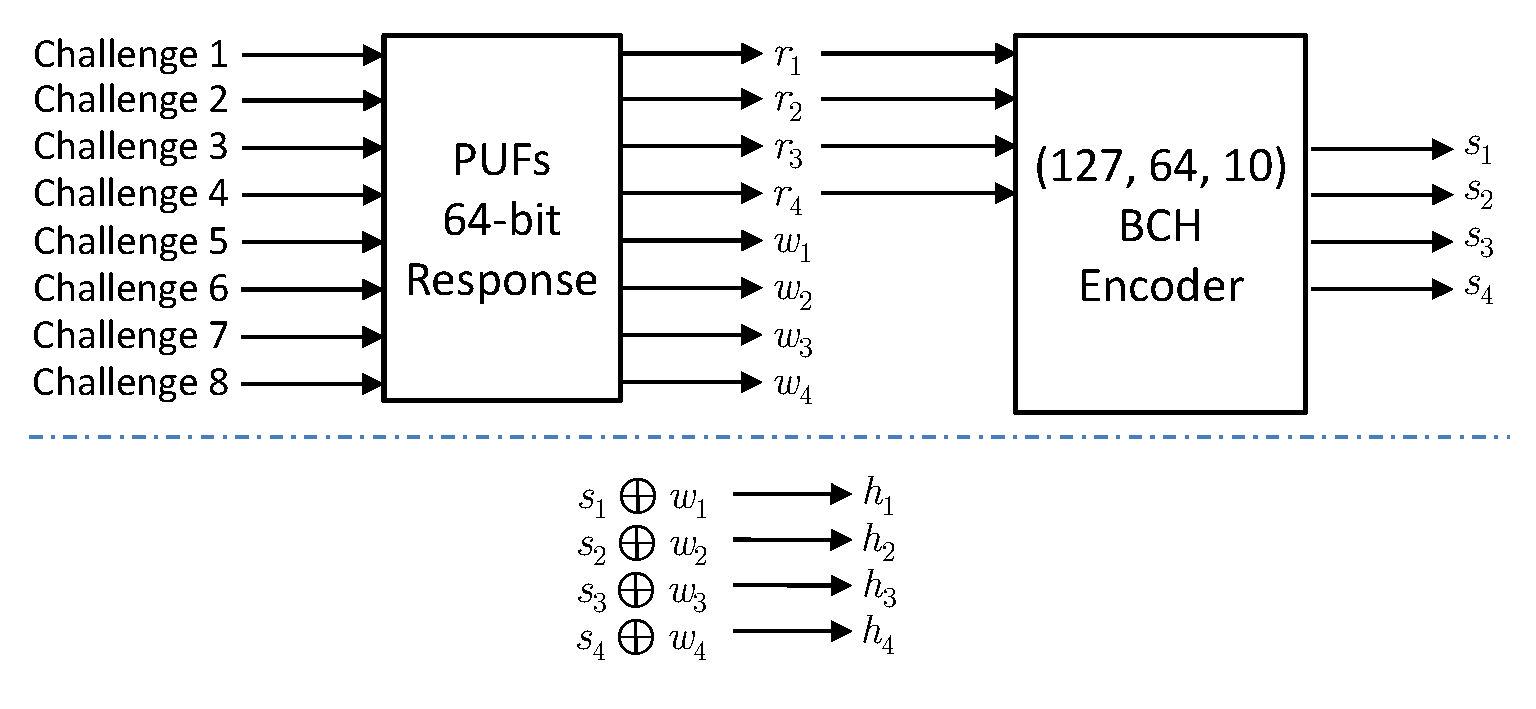
\includegraphics[width=\textwidth]{fuzzy-enroll}
         \caption{\fuzzy~during key extraction.}
         \label{fig:fuzzy-enroll}
     \end{subfigure}
     \hfill
     \begin{subfigure}[b]{0.5\textwidth}
         \centering
         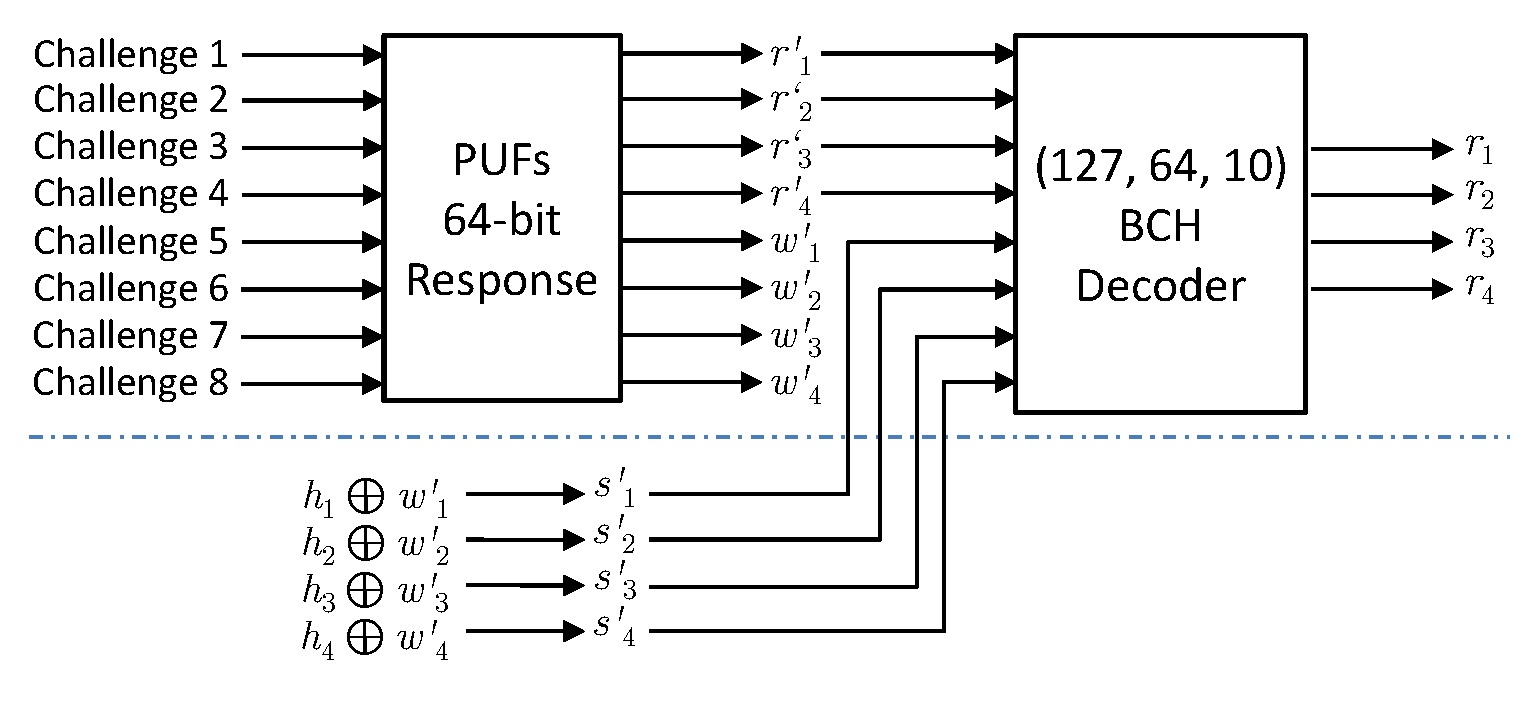
\includegraphics[width=\textwidth]{fuzzy-regen}
         \caption{\fuzzy~during key regeneration.}
         \label{fig:fuzzy-regen}
     \end{subfigure}

        \caption{\fuzzy~actions during the enrollment and recovery procedure.}
        \label{fig:fuzzy-extractor}
\end{figure}

To fully explain \fenroll, the chosen parameters are detailed. First, \cshia~incorporates \pufs~that produce 64-bit responses. These \pufs~ will be responsible for generating each string $r$ and $w$ that are 64 bits long. To match the length of $r$ and $w$, \cshia~has a $(127, 64, 10)$-\bch~\ecc. As \fenroll~depicts, there are four-bit strings $r_i$, which are compounded two by two and fed to the \prf~(Figure \ref{fig:key-construction}). Such combinations were specifically designed to match the \prf~chosen for \cshia, the \siphash~\cite{Aumasson2012:SipHash}, which has an output of 64 bits and uses a key of 128 bits. Therefore, the first pair of bit strings $r_i$ is concatenated with a constant and processed by the \prf~using the second pair of bit string $r_i$ as key. That generates a hash $K_1$. Then, inverting their places and concatenating the second pair with a different constant, a hash $K_2$ is obtained. Concatenating $K_1$ with $K_2$ results in $K$ which is the secret key of \cshia. Notice that $C_1$ and $C_2$ in Figure \ref{fig:key-construction} are replacing addresses for input of the \ptaggen. One can notice that assuming that each bit string $r_i$ has at least half of their length of entropy, each part of the key will have full entropy. Hence, the key has full entropy. 

\subsubsection{Full Memory Protection}
\label{subsubsec:Full-Memory-Protection}

The Enrollment Phase proceeds to tag the memory range the manufacturer\slash{}vendor specified during design. Now that \ptaggen~has a unique key, \seceng~orders \handler~to bring all memory blocks and deliver them to it. \seceng~will use \ptaggen~to generate \ptags.%, however, depending on the solution against replay attacks a designer chooses, \ptaggen~is used differently. 

% \paragraph{Timestamps Generation}
% \label{paragraph:Timestamps-Generation}

% When timestamps are the solution against replay attacks, \pmmu~will have a timestamp memory. This timestamp memory has the depth of the number of data memory blocks the designer chose to cover. Thus, before \handler~hands in data memory blocks, \pmmu~will clear the entire timestamp memory to avoid uninitialized values. While \seceng~receives code memory blocks, generated \ptags~are just passed to \pmmu~that stores them in \ptagmem. As \handler~starts to pass data memory blocks to \seceng, \pmmu~increments the timestamp of each memory block received and passes this value to \seceng, which combines with the address of the memory block. This combination is then concatenated with the memory block and then finally hashed into a \ptag. \pmmu~receives this \ptag~and stores it in \ptagmem.

% \paragraph{\mt~Generation}
% \label{paragraph:Merkle-Tree-Generation}

% A \mt~solution is more complex. The first procedure is very straightforward. \seceng~receives memory blocks and their addresses from \handler~and uses \ptaggen~to generate \ptags. \pmmu~receives these \ptags~and sends them to \ptagmem. After all memory blocks had their \ptags~generated, \pmmu~starts to bring \ptags~of data memory blocks. As soon as a chunk of \ptags~is formed, a \ptag~internal address of the chunk is calculated. \pmmu~provides this internal address and the chunk to \ptaggen~that generates a \ptag. This \ptag~is returned to \pmmu~that stores it in \ptagmem. This process will continuously happen (as we can see in Figure \ref{fig:vtree}) until \pmmu~identify that the last \ptag~calculated has no siblings. Hence, it is the root \ptag, which must be stored inside \pmmu. It is worth to clarify that \ptag~internal address is an address space that facilitates computation and identification of descendants and ancestors. Each internal address is directly translated to a physical address by \pmmu~and this translation has as goal to minimize unused spaces in \ptagmem. Moreover, in terms of security, this internal address mitigates a very specific attack on the tree, in which an descendant has the same \ptag~as one of its ancestors. In this case, an attacker could try to perform a relocation attack likewise. 
